\documentclass[conference]{IEEEtran}
\IEEEoverridecommandlockouts
% The preceding line is only needed to identify funding in the first footnote. If that is unneeded, please comment it out.
\usepackage{cite}
\usepackage{amsmath,amssymb,amsfonts}
\usepackage{algorithmic}
\usepackage{graphicx}
\usepackage{textcomp}
\usepackage{diagbox}
\usepackage{subfigure}
\usepackage{xcolor}
\def\BibTeX{{\rm B\kern-.05em{\sc i\kern-.025em b}\kern-.08em
    T\kern-.1667em\lower.7ex\hbox{E}\kern-.125emX}}
\begin{document}

\title{Feature Encoding for Image Classification\\
%{\footnotesize \textsuperscript{*}Note: Sub-titles are not captured in Xplore and
%should not be used}
%\thanks{Identify applicable funding agency here. If none, delete this.}
}

\author{\IEEEauthorblockN{Haowei Huang}
\IEEEauthorblockA{\textit{516021910491} \\
\textit{Shanghai Jiao Tong University}\\
Shanghai, China \\
1270927224@qq.com}
\and
\IEEEauthorblockN{Zhixin Lin}
\IEEEauthorblockA{\textit{516021910495} \\
\textit{Shanghai Jiao Tong University}\\
Shanghai, China \\
1069066484@qq.com}
\and
\IEEEauthorblockN{Yaojie Ding}
\IEEEauthorblockA{\textit{516021910430} \\
\textit{Shanghai Jiao Tong University}\\
Shanghai, China \\
416914846@qq.com}
}

\maketitle

\begin{abstract}
Abstract of Project4.
\end{abstract}



\section{Introduction}
Introduction of Project4.


\section{Approaches}
In this section, we present our methods applied for classification. And we will emphasize differences of our approaches compared with standard ones.

\subsection{ADDA}
Eric Tzeng, et al. summarized a generalized architecture for adversarial domain adaptation and introduced a method of domain adaptation, Adversarial Discriminative Domain Adaptation, in his work \cite{ADDA1}. Using their summarization, ADDA is a combination of generative and discriminative neural network model that uses untied weight sharing between source mapping and target mapping and a GAN loss.

\begin{figure*}
  \centering
  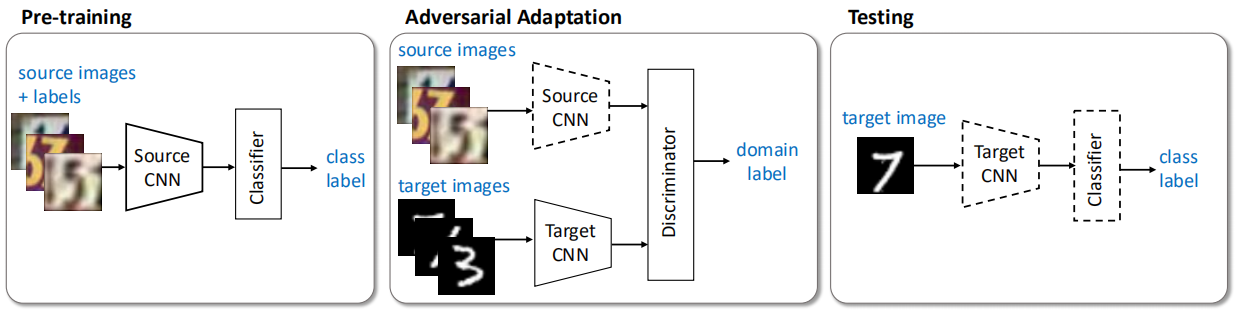
\includegraphics[width=.75\textwidth]{LADDA_theorem1.jpg}
  \caption{ADDA Overview: An overview of standard ADDA architecture. Dashed lines indicate fixed network parameters in the indicated stage.}
  \label{ADDA_overview}
\end{figure*}
The general ADDA approach is presented in figure \ref{ADDA_overview}. There are overall four relatively separated subnetworks within the ADDA model:
\begin{enumerate}
  \item Source encoder network, $M_s$. Source encoder take source data set as input and output the encoded source features.
  \item Target encoder network, $M_t$. Target encoder take source data set as input and output the encoded target features.
  \item Discriminator network, $D$. Discriminator take encoded source features and encoded target features and tries to identify which come from source dataset and target dataset.
  \item Classifier network, $C$. Classifier network take encoded features, from either source or target domain, as input and output the class prediction.
\end{enumerate}

According to work of Eric Tzeng, et al., we can divide the way the model runs into three stages:
\begin{enumerate}
  \item Pre-training. In this stage, we feed source training data, $X_{s}$ for source encoder network and use the output features, $M_s(X_{s})$, to feed classifier network and use cross entropy as classification loss , $L_{c}$:
      \begin{equation}\label{cls_loss}
      \begin{aligned}
        L_{c} & (X_{s}, Y_{s}) =  \\
        &-\mathbb{E}_{(x_s,y_s) \sim (X_s,Y_s)}
        \sum\limits_{k=1}^{K} \mathbb{I}_{[k=y_s]} \log C(M_s(X_{s}))
        \end{aligned}
      \end{equation}
       to train the source network and classifier network. After that, both source network and classifier network are fixed. $K$ is the total number of classes.
  \item Adversarial adaptation. In this stage, we use the idea of GAN to train $M_t$ to generate features, $M_t(X_{t})$, to be similarly distributed as $M_s(X_{s})$. We feed $X_s$ and $X_t$ for $M_s$ and $M_t$ respectively and combination of $M_s(X_{s})$ and $M_t(X_{t})$ for $D$. We in turn optimize $D$ to minimize $L_{D}$:
      \begin{equation}\label{LD}
        \begin{aligned}
        L_{D} & (X_{s}, X_{t}, M_s, M_t) =  \\
                                        &-\mathbb{E}_{(x_s) \sim (X_s)} \log D(M_s(X_{s})) \\
                                        &-\mathbb{E}_{(x_t) \sim (X_t)} \log (1 - D(M_t(X_{t}))
            \end{aligned}
      \end{equation}
      and optimize $M_t$ to minimize
      $L_{t}$:
      \begin{equation}\label{Lt}
        L_{t}(X_{s}, X_{t}, D) =
            -\mathbb{E}_{(x_t) \sim (X_t)} \log D(M_t(X_{t}))
      \end{equation}
      $D$ tries to distinguish $M_s(X_{s})$ and $M_t(X_{t})$ while $M_t$ want to deceive $D$. \\
      Our approach is not always quite standard as Eric Tzeng's work. Except that we use fully connected layers instead of CNN for our $X_s$ and $X_t$, we also initialized parameters of $M_t$ using pre-trained $M_s$'s. This is not mentioned in the paper and it is not likely to be feasible in most cases. We can do so because our structure of $M_s$ is designed to be the same as $M_t$. And the measure really help a lot.
  \item Testing. In this stage, we feed $M_t(X_t)$ for $C$ and evaluate the classification accuracy.
\end{enumerate}
    With our practice, we combined the last two stages into one, just say adversarial adaptation. ADDA method is just like trying to encode the target domain data, $M_t(X_t)$, to match the distribution of encoded source domain data, $M_s(X_s)$ so that the classifier working on source domain data can also work on target domain data.




\subsection{DANN}
Yaroslav Ganin, et al. proposed a representation learning approach for domain adaptation in their work \cite{DANN1}. DANN can also be viewed as an instance of Eric Tzeng, et al.'s summarization of domain adaptation method. Compared with ADDA, in general, the only difference of DANN is that DANN is an architecture of tied weight sharing.
\begin{figure*}
  \centering
  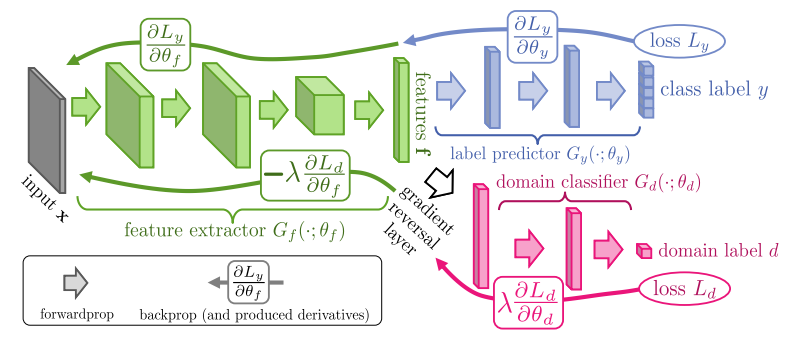
\includegraphics[width=.8\textwidth]{LDANN_theorem1.jpg}
  \caption{DANN Overview: An overview of standard DANN architecture.}
  \label{DANN_overview}
\end{figure*}
The general architecture is presented in figure \ref{DANN_overview}; it's simpler than ADDA. Domain classifier $D$ of DANN performs similar function as discriminator $D$ of ADDA does. DANN is similar to ADDA but target encoder and source encoder share the same weight weights. In other words, only one feature encoder, $M$, is used within DANN. Thus, we do not go to details of components of DANN and just simply present the way the DANN model work. We will use similar representations as ADDA to make things easy to understand (although they may not be Yaroslav Ganin et al.'s symbols).
\begin{enumerate}
  \item Pre-training. In this stage, we optimize $M$ and $C$ to minimize $L_{C}$.
  \item Adversarial adaptation. In this stage, we feed both $X_s$ and $X_t$ for $M$. By fixing $C$, we optimize $M$ and $D$ to minimize $L_{da}$:
      \begin{equation}\label{dann_da}
        \begin{aligned}
        L_{da} & (X_{s}, X_{t}, M) =  \\
                            &-(\mathbb{E}_{(x_s) \sim (X_s)} \log D(M(X_{s})) \\
                            &+\mathbb{E}_{(x_t) \sim (X_t)} \log (1 - D(M(X_{t}))) \times c_{da} \\
                            &-\mathbb{E}_{(x_s,y_s) \sim (X_s,Y_s)}
                            \sum\limits_{k=1}^{K} \mathbb{I}_{[k=y_s]} \log C(M(X_{s}))
        \end{aligned}
      \end{equation}
      Unlike ADDA, parameters of $M$ and $D$ are updated at the same time. And the loss, $L_{da}$ of DANN is combination of both $L_C$ and $L_D$ of ADDA. There is subtle difference between ADDA and DANN in this stage. $C_{da}$ is a balance factor for classification loss and discriminator loss. $c_{da}$ is not mentioned in the paper, but we use it and find it helps improve our model. We use $c_{da}=2.0$.
  \item Testing. In this stage, we feed $M(X_t)$ for $C$ and evaluate the classification accuracy.
\end{enumerate}
Also, we combined stage of adversarial adaptation and testing together as adversarial adaptation. Compared to ADDA method that tries to bring $M_t(X_t)$ to $M_s(X_s)$ as closer as possible, DANN method is just like trying to adjust a well-trained source domain encoder $M_s$ to work on target domain data, $X_t$.

\section{Experiments And Results}
\subsection{ADDA Experiments}
We will present six experiments in this part. We use fully connected networks (FCNs) to construct the four subnetworks. First we show some common parameters of all of these experiments in table \ref{tab:SymADDA}. We split both $X_s$ and $X_t$ into training set, $X^{tr}_s$ and $X^{tr}_t$, and test set, $X^{te}_s$ and $X^{te}_t$. $X^{tr}_s$ is used to train ADDA the first stage and $X^{te}_s$ is used to select the best parameters of $M_s$ and $C$ correspondingly, preventing overfitting. $X^{te}_t$ is used to train ADDA the second stage and $X^{te}_t$ is used to select the best parameters of $M_t$ and $D$ correspondingly, also preventing overfitting. It should be mentioned that both $X^{te}_t$ and $X^{tr}_t$ are unlabeled.
 \begin{table}[h]
	\centering
	\caption{Hyper-parameters of ADDA}
	\label{tab:SymADDA}
	\begin{tabular}{ccc}
		\hline
		Symbol & Value & Description \\
		\hline
		\hline
        $K$ & $65$ & Number of classes \\
		$s$ & $5e-5$ & Optimization step \\
		$b$ & $256$ & Batch size \\
		$l_e$ & ${2048,2048}$ & Layers of $M_s$ and $M_t$ \\
		$l_c$ & ${1024,K}$ & Layers of $C$, connected from o$M_c$ or $M_t$  \\
		$l_d$ & ${512,512,2}$ & Layers of $D$, connected from $M_c$ or $M_t$ \\
        $p_k$ & $0.05$ & Dropout probability of a neuron. \\
        $l_2$ & $1e-5$ & L2 regularization for weight parameters.  \\
        $r^{tr}_{s}$ & $0.9$ & Ratio of $X_s$ used as training set.\\
        $r^{tr}_{t}$ & $0.6$ & Ratio of $X_t$ used as training set.  \\
        $I$ & $8000$ & Total iterations of first two training stages.   \\
		\hline
	\end{tabular}
\end{table}

 \begin{table*}[h]
	\centering
	\caption{Different Configurations And Resulted Performances of ADDA Experiments}
	\label{tab:ConfigADDA}
	\begin{tabular}{cccccccccc}
		\hline
		Sym & Src & PT & AN & BN & $Ac(M_s(X^{te}_s))^*$ & $Ac(M_s(X^{te}_t))^*$ & $Ac(M_t(X^{tr}_t))^*$ & $Ac(M_t(X^{te}_t))^*$ & g\\
		\hline
		\hline
        $Ex1$ & Art & $\times$ & $\times$ & $\times$ & 0.6074 & 0.5080 & 0.0222 & 0.0189  & -0.4891\\
		$Ex2$ &  Art & \checkmark & $\times$ & $\times$ & 0.6818 & 0.5712 & 0.5897 & 0.5821 & 0.0109\\
		$Ex3$ &  Art & \checkmark & \checkmark & $\times$ & 0.6488 & 0.6223 & 0.6551 & 0.6372 & 0.0149\\
		$Ex_A$ &  Art & \checkmark & \checkmark & \checkmark & 0.7893 & 0.7313 & 0.7621 & 0.7354 & 0.0041\\
		$Ex_C$ &  Clipart & \checkmark & \checkmark & \checkmark & 0.8624 & 0.6561 & 0.6646 & 0.6636 & 0.0075\\
		$Ex_P$ &  Product & \checkmark & \checkmark & \checkmark & 0.9391 & 0.7313 & 0.7556 & 0.7353 & 0.0040\\
		\hline
	\end{tabular}
\end{table*}
Then we present a overview of different configurations of the six experiments and the corresponding results in table \ref{tab:ConfigADDA}. Target domain of all of the experiments presented is real world. Src is short for source data domain. PT stands for whether to transfer parameters of $M_s$ to $M_t$ for $M_t$'s initialization. AN means whether to apply learning rate annealing. BN means whether to apply batch normalization for each layer. Besides, we uses RELU function for hidden layer's activation and adds a softmax layer before calculating cross entropy. With learning rate annealing applied, we have learning rate of stage pre-training and adversarial adaptation to be $l_{r1}=\frac{1.5 \times s}{1.0 + 0.01 \times i}$ and $l_{r2}=\frac{0.1 \times s}{1.0 + 0.01 \times i}$, where $i$ it the iteration number. Otherwise, $l_{r1}=s$ and $l_{r2}=0.05 \times s$. We acquired these formulas by preliminary experiments.

$Ac(x)^*$ indicates the best accuracy towards indicator $x$. For example, in the formula $Ac(M_t(X^{te}_t))^*$, $X^{te}_t$, $M_t$ and $Ac^*$ stands for test set of unlabeled target domain, target encoder and the best accuracy respectively. Thus, $Ac(M_t(X^{te}_t))^*$ means the best test classification accuracy towards target test set using target encoder. $Ac(M_t(X^{te}_t))^*$ is actually the final classification evaluation of our domain adaptation method. Similarly, $Ac(M_s(X^{te}_s))^*$ represents the best accuracy of the classifier towards source test dataset using source encoder, which can be viewed as an upper bound of $Ac(M_t(X^{tr}_t))^*$. $Ac(M_t(X^{tr}_t))^*$ represents the best accuracy of the classifier towards target training dataset using target encoder, which also can be viewed as an upper bound of $Ac(M_t(X^{te}_t))^*$. So, we theoretically have $Ac(M_s(X^{te}_s))^* \geq Ac(M_t(X^{tr}_t))^* \geq Ac(M_t(X^{te}_t))^*$ . As for $Ac(M_s(X^{te}_t))^*$, it represents the best accuracy of the classifier towards target test dataset using source encoder. We can use $g=Ac(M_t(X^{te}_t))^*-Ac(M_s(X^{te}_t))^*$ as the performance gain with our domain adaptation method.

Now, we go to details of the six experiments. The figures \ref{fig:Ex1}, \ref{fig:Ex2}, \ref{fig:Ex3}, \ref{fig:ExA}, \ref{fig:ExC} and \ref{fig:ExP} show visualization of the results. Four each figure, there are four subfigures showing target dataset  distribution before and after domain adaptation, classifier training history in stage pre-training, discriminator training history in stage adversarial adaptation and accuracies of $X_t$ changing in stage adversarial adaptation. Remember we combine test stage into adversarial adaptation stage. In the fourth subfigure, acc(t\_ec, training set), acc(t\_ec, test set), acc(s\_ec, training set), acc(s\_ec, test set) stands for $Ac(M_t(X^{tr}_t))$, $Ac(M_t(X^{te}_t))$, $Ac(M_s(X^{tr}_t))$ and $Ac(M_s(X^{te}_t))$ respectively. And all values of the loss curves are scaled to interval $[0.0, 1.0]$ for a better observation.

As illustrated in figure \ref{fig:Ex1}, the domain adaptation just shows no effect($Ac(M_t(X^{te}_t))^* < 0.03$). We would rather use the source encoder $M_s$ for our target dataset and achieves a test accuracy above 0.50. We tried Ex1 exactly the same as Eric Tzeng st al.'s work. Just we are using features of images instead of images themselves(Maybe we missed something in the paper). By observing transfer visualization(the first subfigure), the adapted target data just moved to another distribution and still obviously separated from the source data. By observing discriminator's training history(the third subfigure), we can see the discriminator loss falls fast and within 800 iterations, the discriminator can successfully distinguish $M_t(X_t)$ and $M_s(X_s)$ no matter how $M_t$ is trained. Thus, we believe it must be that a randomly initialized $M_t$ parameters are too chaotic for $M_t$ to optimize and deceive the discriminator.

To fix the problem, we decided to initialize $M_t$ parameters with trained $M_s$'s since we think the object features from source and target domain must have a lot in common and $M_t$ can be adjusted from $M_s$. As illustrated in figure \ref{fig:Ex2}, the result is much better. From discriminator's training history, we see GAN training curves. There exists a negative correlation between $L_D$ and $L_t$, represented by the blue and orange curve in the third subfigure respectively. In this experiment, the $Ac(M_t(X^{te}_t))^*$ overcomes $Ac(M_s(X^{te}_t))^*$ by about 0.01. The domain adaptation shows a positive effect. But, we found a problem that, in the stage of adversarial adaptation, $Ac(M_t(X^{te}_t))$, represented by the orange curve in the fourth subfigure, drops quickly at first(though increases then). And we found this is not a corner case, Eric Tzeng et al. mentioned the problem on the internet and suggested we try decreasing the learning rate.

So we have Ex3, shown in \ref{fig:Ex3}, we applied method of learning rate annealing. The process of $C$'s training in the pre-training stage(the second subfigure) improves a lot. It also help ease dropping of $Ac(M_t(X^{te}_t))$. However, still we found the training processes converge too slow in both stages. The $C$ doesn't seem to converge even after 8000 iterations.

To solve the problem, we tried method of batch normalization, as illustrated in \ref{fig:ExA}. The training of classifier $C$ converges within 800 iterations, far more quickly than before. Discriminator's training becomes more gently although $D$ grows too powerful for $M_t$ to deceive. And $Ac(M_t(X^{te}_t))^*$ grows to be 0.7354, far better than the previous three experiments. We are using the same dataset in the four experiments so far.

We show figures \ref{fig:ExC} and \ref{fig:ExP} for completeness of our study. It seems domain adaptation does not work so well when it comes to transfer art dataset into real world dataset compared to clipart and product dataset thought the classifier works the best on the source dataset. We think it is because there exists a larger different between the two domains, real world and clipart.
\begin{figure*}[htb]

\centering
\begin{minipage}[t]{0.26\textwidth}
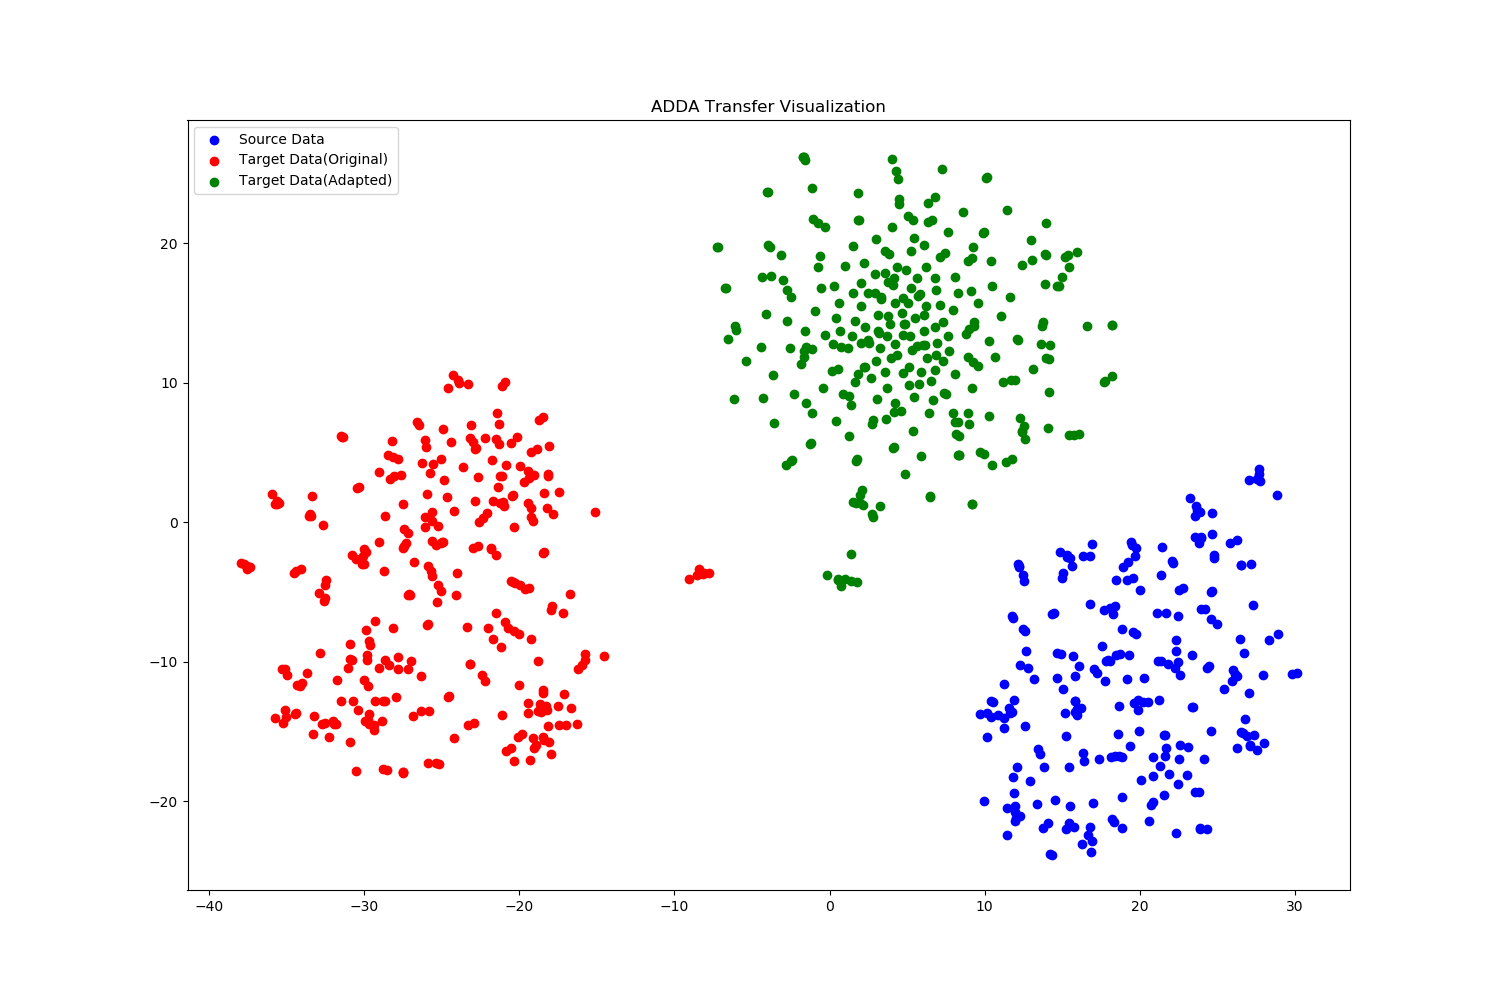
\includegraphics[width=1.6in, height=1.5in]{Ladda/A2R_no_preassign_no_dec_no_bn/ADDA_visual.png}
\end{minipage}%
\begin{minipage}[t]{0.26\textwidth}
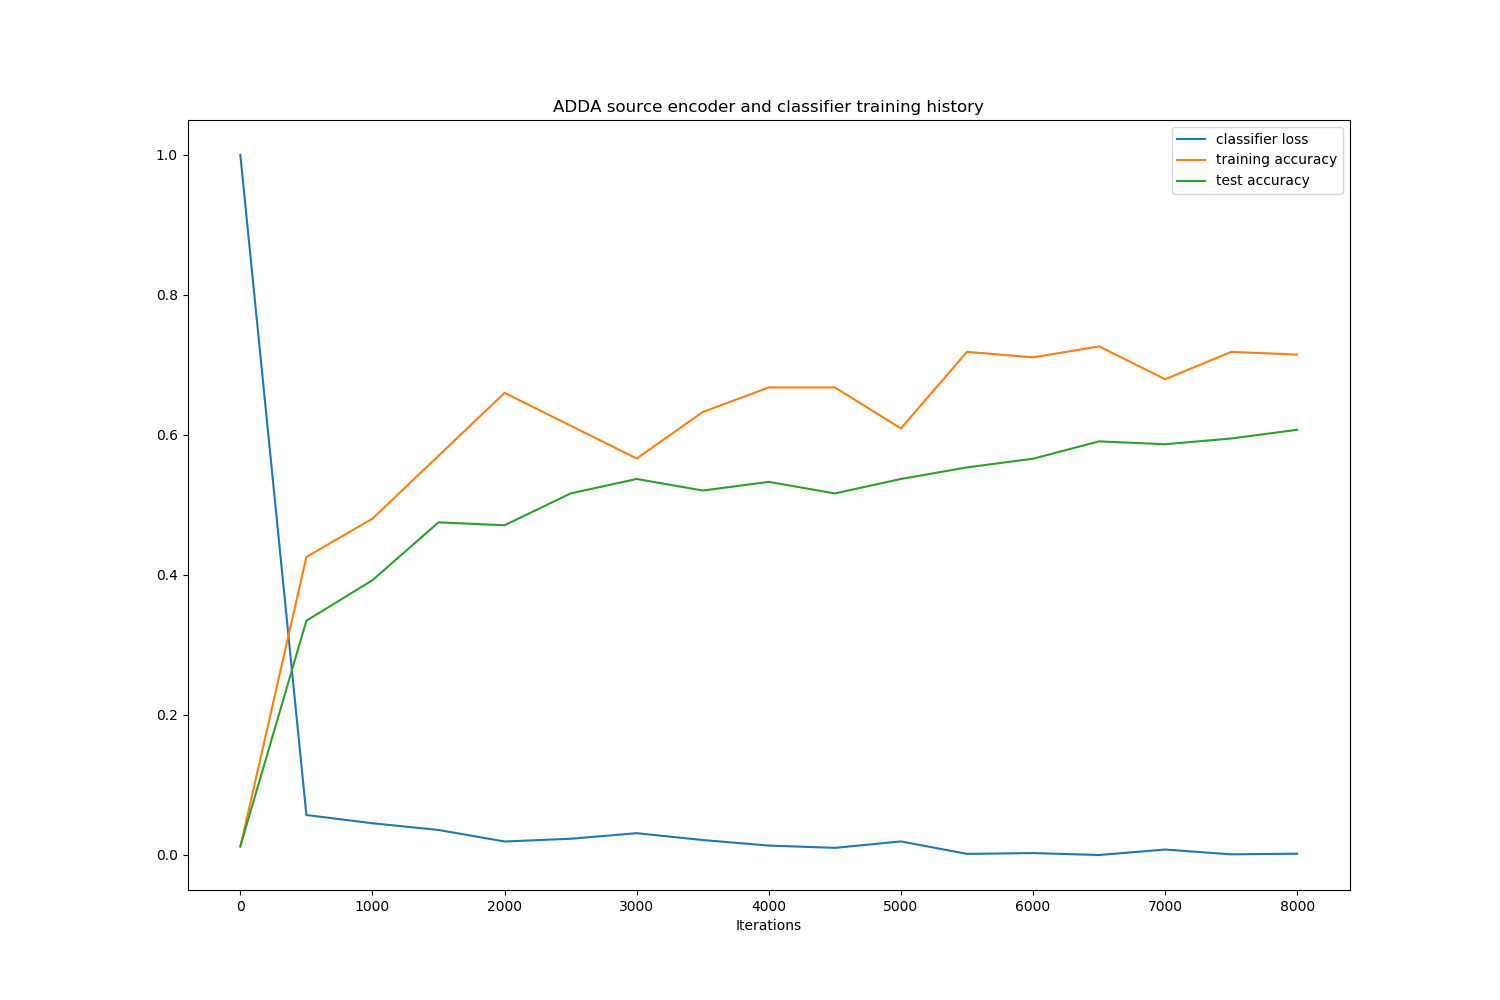
\includegraphics[width=1.6in, height=1.5in]{Ladda/A2R_no_preassign_no_dec_no_bn/clf.png}
\end{minipage}%
\begin{minipage}[t]{0.45\textwidth}
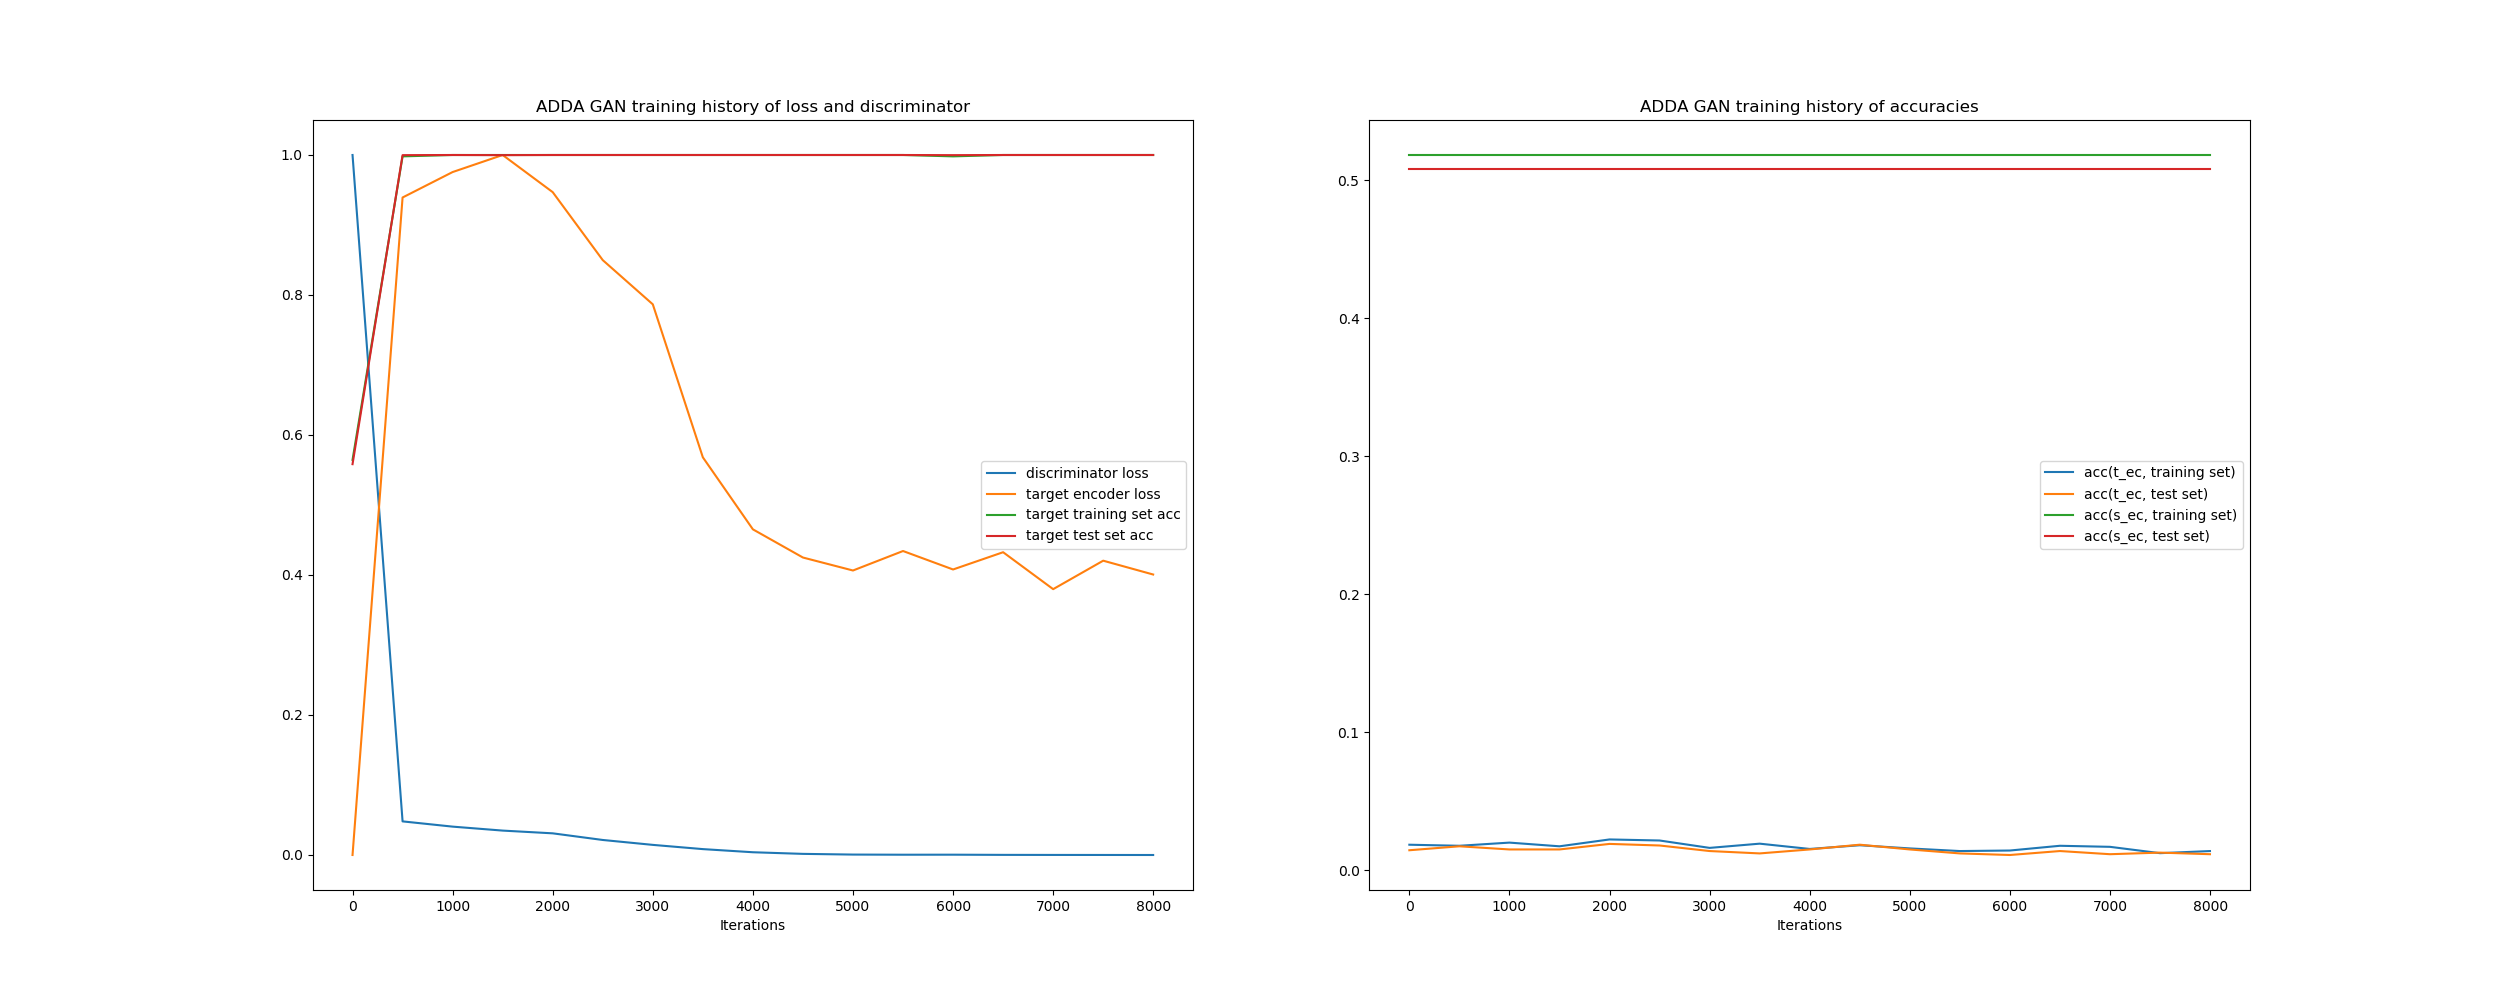
\includegraphics[width=3.5in, height=1.5in]{Ladda/A2R_no_preassign_no_dec_no_bn/gan.png}
\end{minipage}%
\caption{Visualization of ADDA Ex1 Result}\label{fig:Ex1}
\end{figure*}

\begin{figure*}[htb]

\centering
\begin{minipage}[t]{0.26\textwidth}
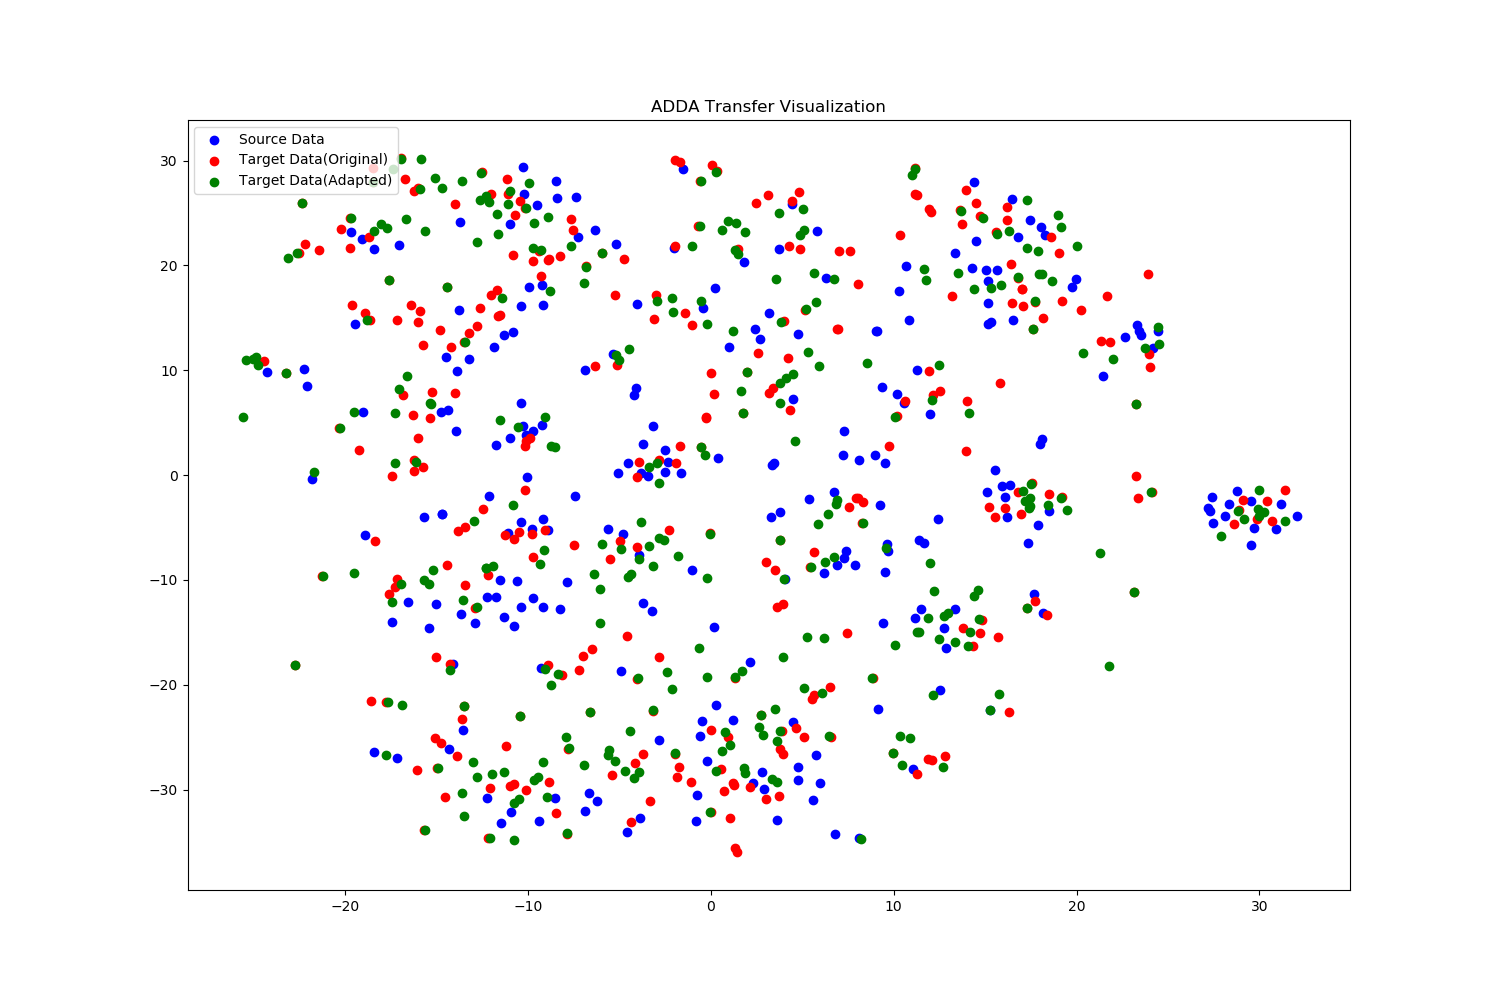
\includegraphics[width=1.6in, height=1.5in]{Ladda/A2R_no_dec_no_bn/ADDA_visual.png}
\end{minipage}%
\begin{minipage}[t]{0.26\textwidth}
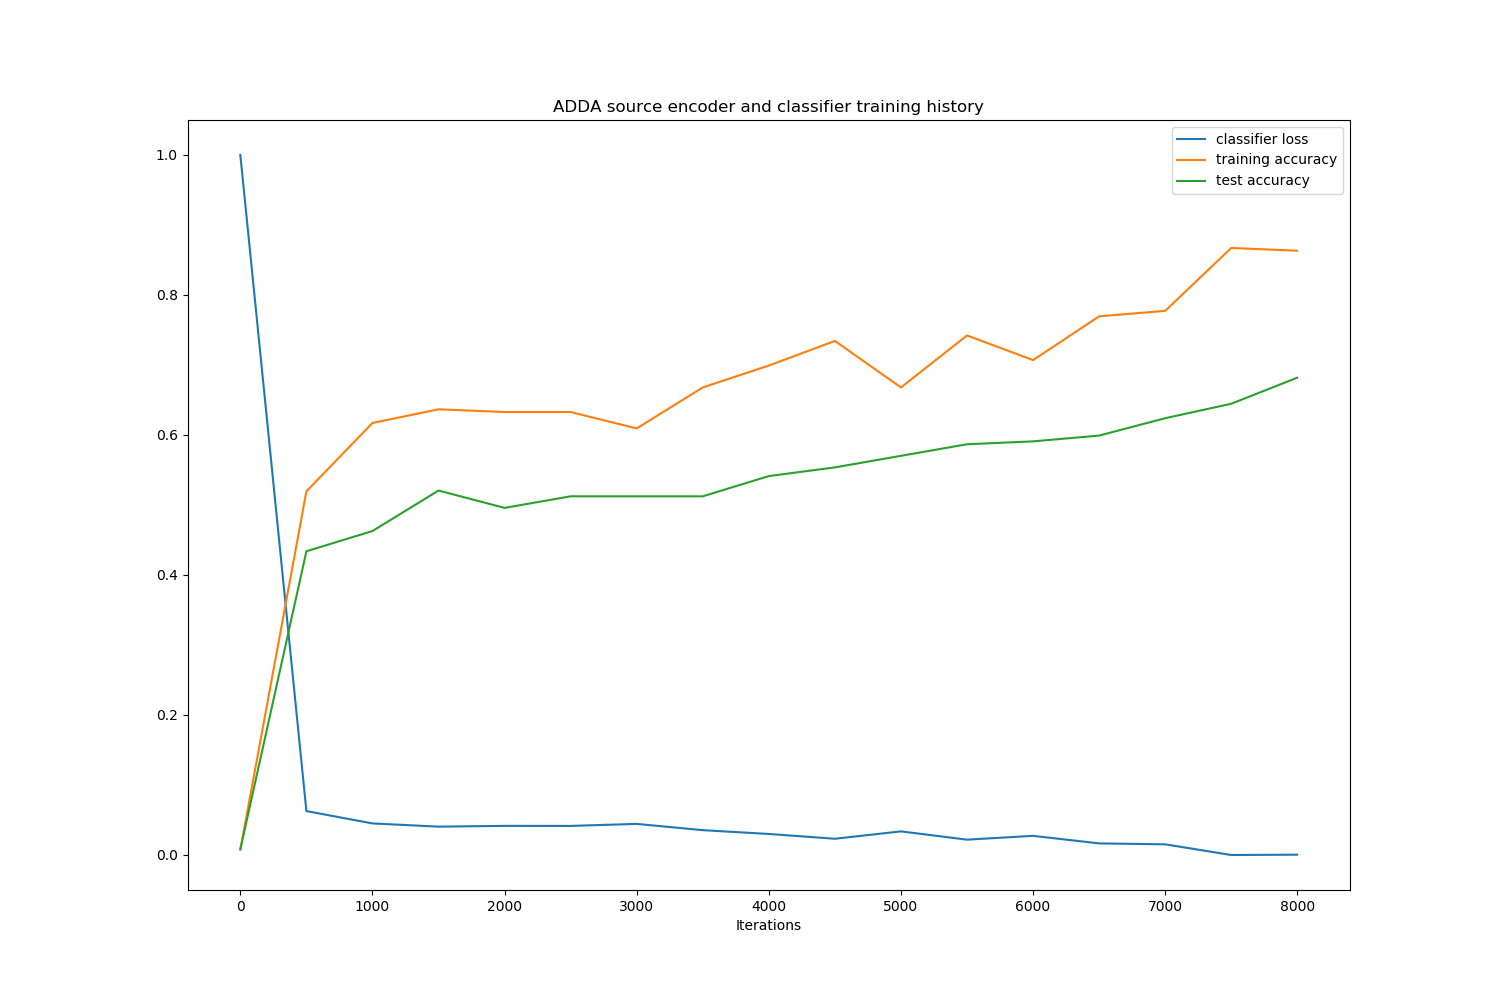
\includegraphics[width=1.6in, height=1.5in]{Ladda/A2R_no_dec_no_bn/clf.png}
\end{minipage}%
\begin{minipage}[t]{0.45\textwidth}
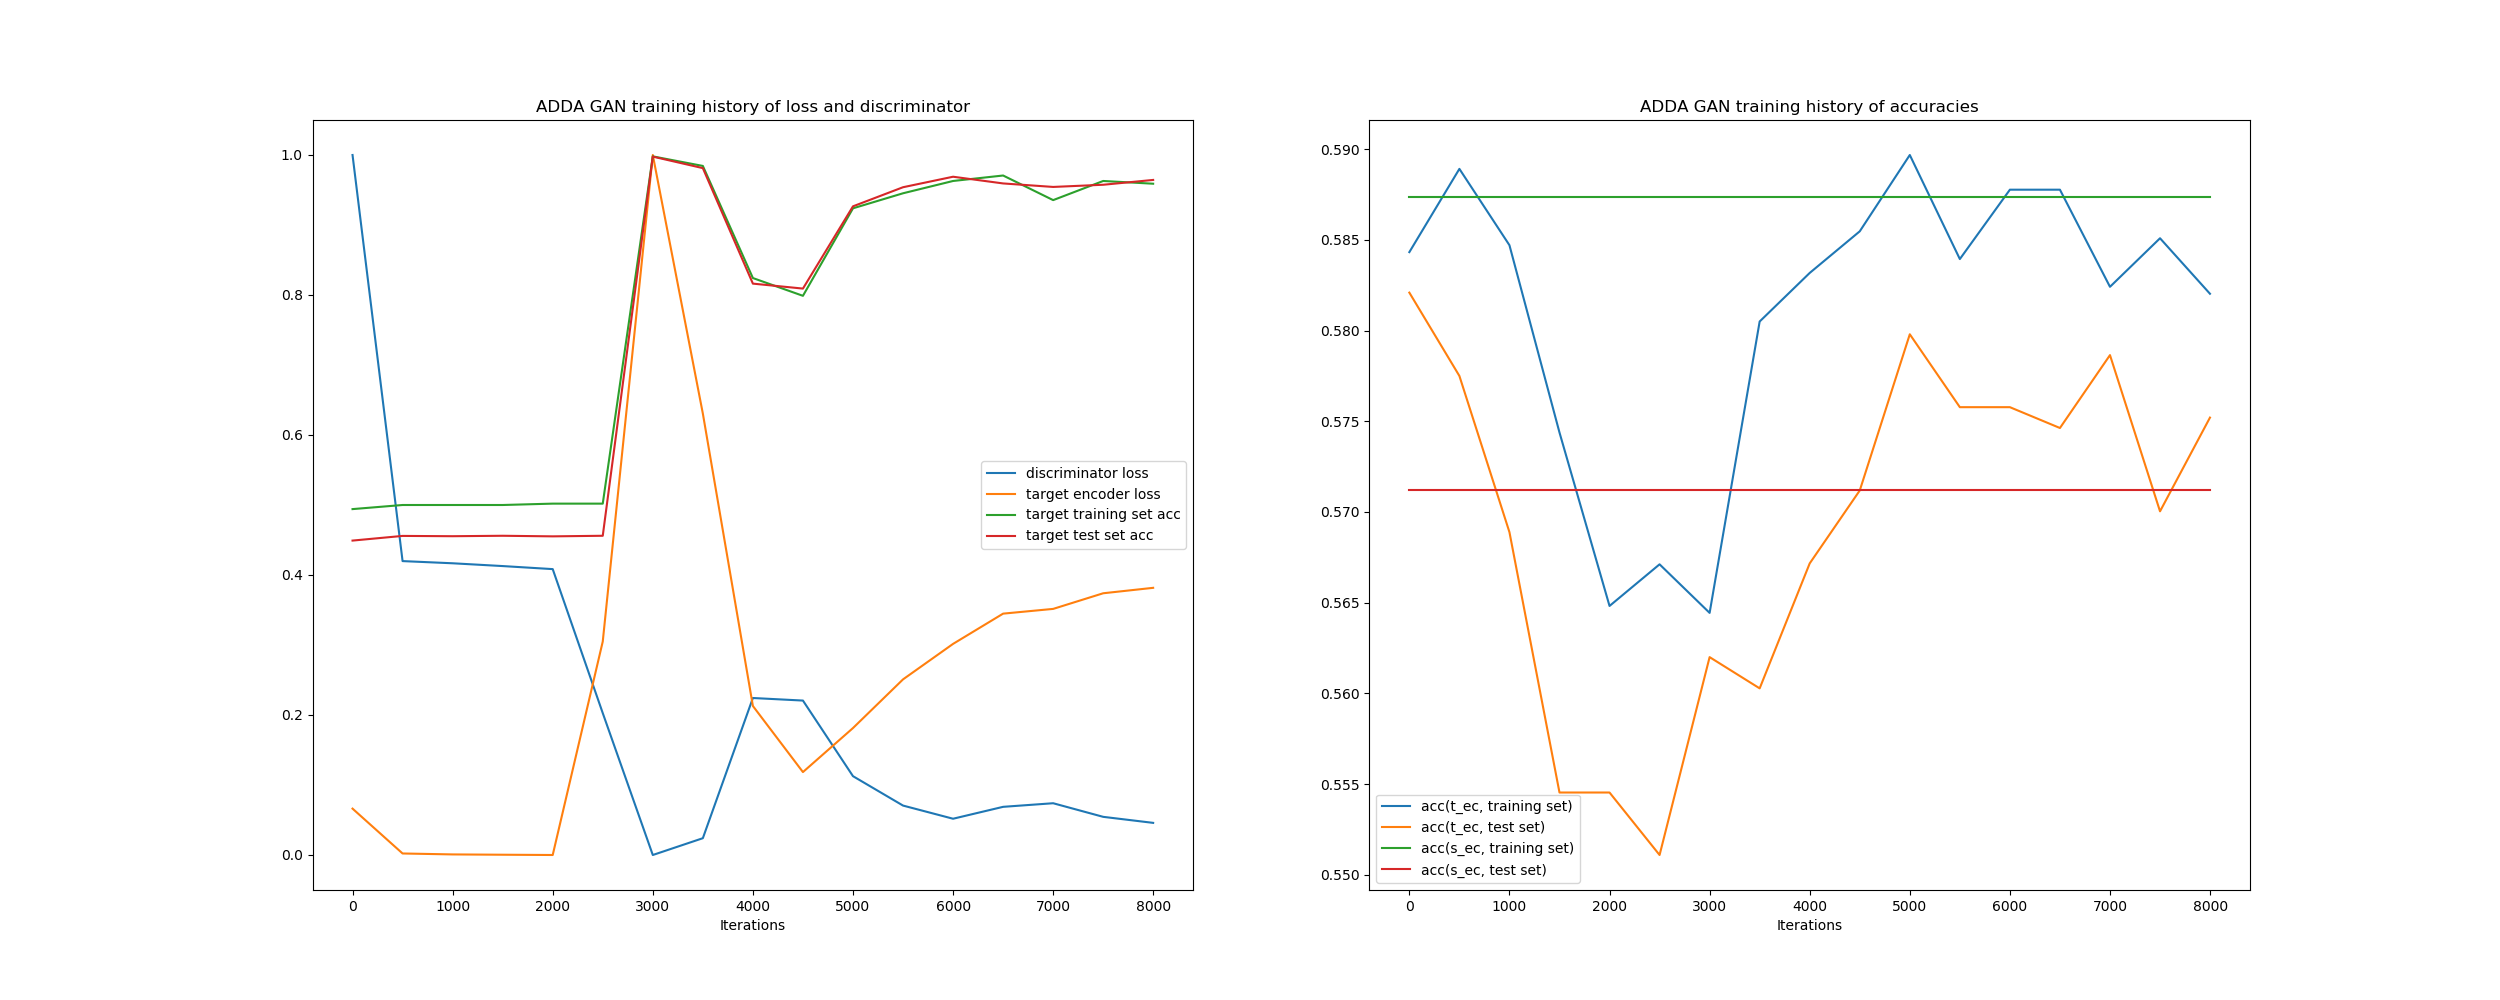
\includegraphics[width=3.5in, height=1.5in]{Ladda/A2R_no_dec_no_bn/gan.png}
\end{minipage}%
\caption{Visualization of ADDA Ex2 Result}\label{fig:Ex2}
\end{figure*}

\begin{figure*}[htb]

\centering
\begin{minipage}[t]{0.26\textwidth}
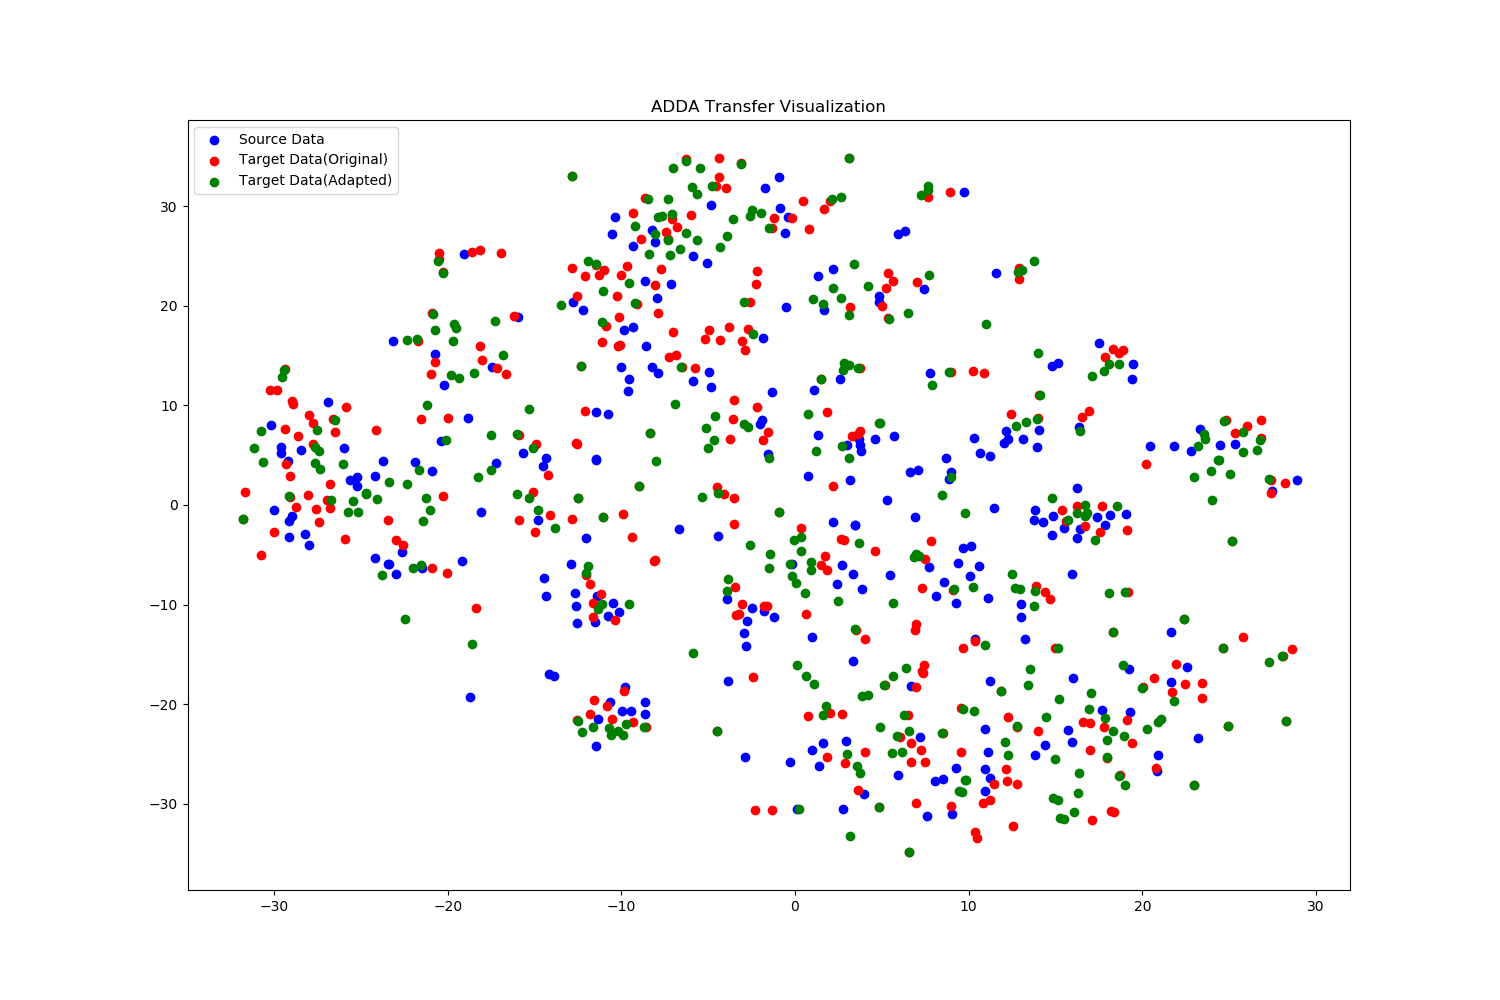
\includegraphics[width=1.6in, height=1.5in]{Ladda/A2R_no_bn/ADDA_visual.png}
\end{minipage}%
\begin{minipage}[t]{0.26\textwidth}
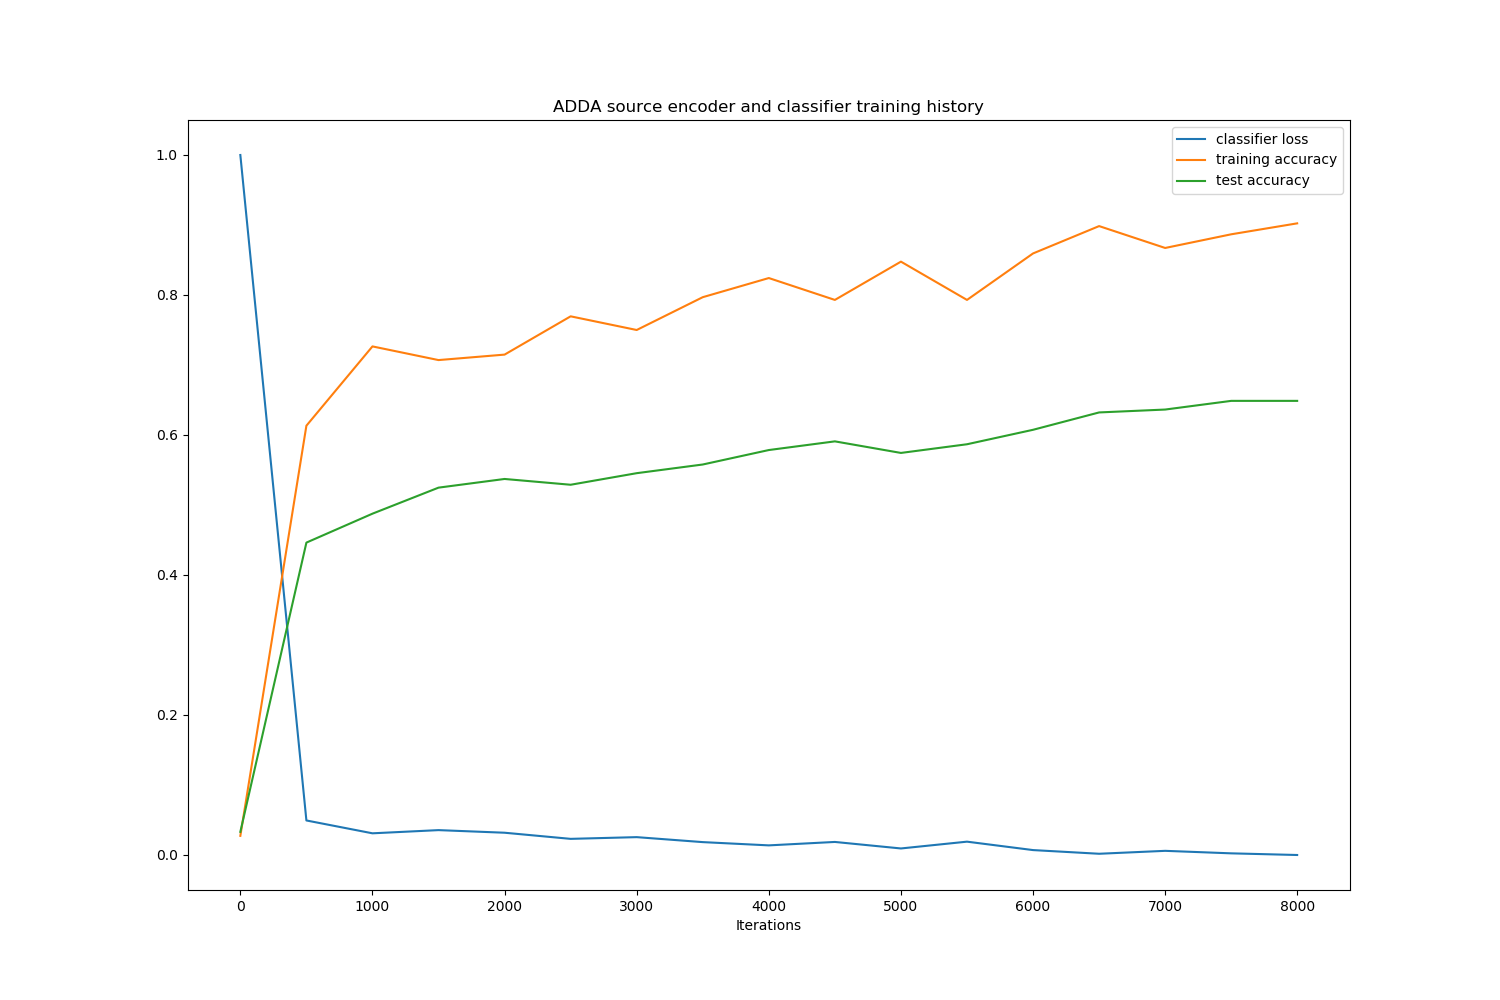
\includegraphics[width=1.6in, height=1.5in]{Ladda/A2R_no_bn/clf.png}
\end{minipage}%
\begin{minipage}[t]{0.45\textwidth}
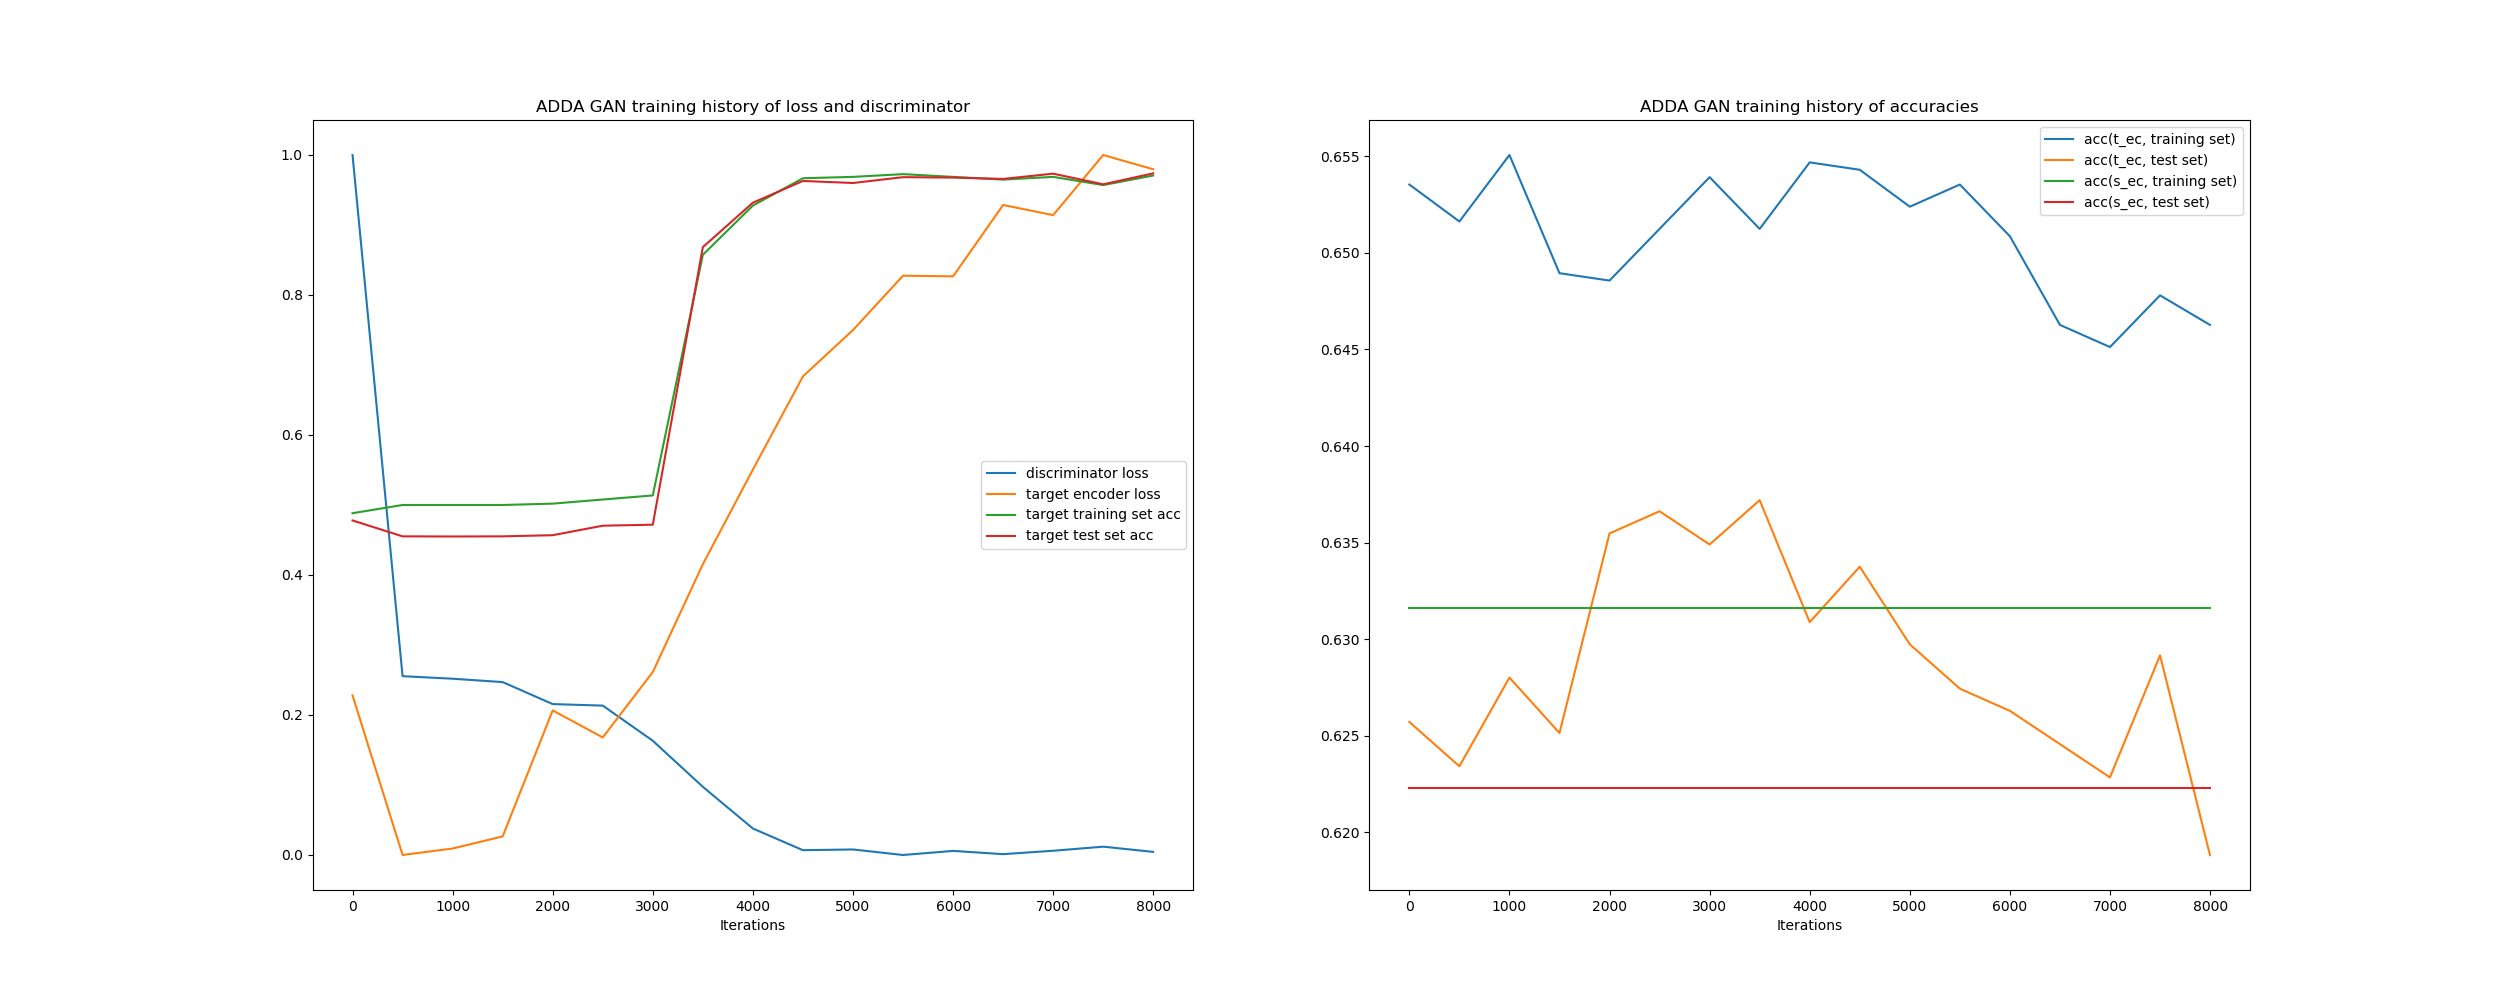
\includegraphics[width=3.5in, height=1.5in]{Ladda/A2R_no_bn/gan.png}
\end{minipage}%
\caption{Visualization of ADDA Ex3 Result}\label{fig:Ex3}
\end{figure*}

\begin{figure*}[htb]

\centering
\begin{minipage}[t]{0.26\textwidth}
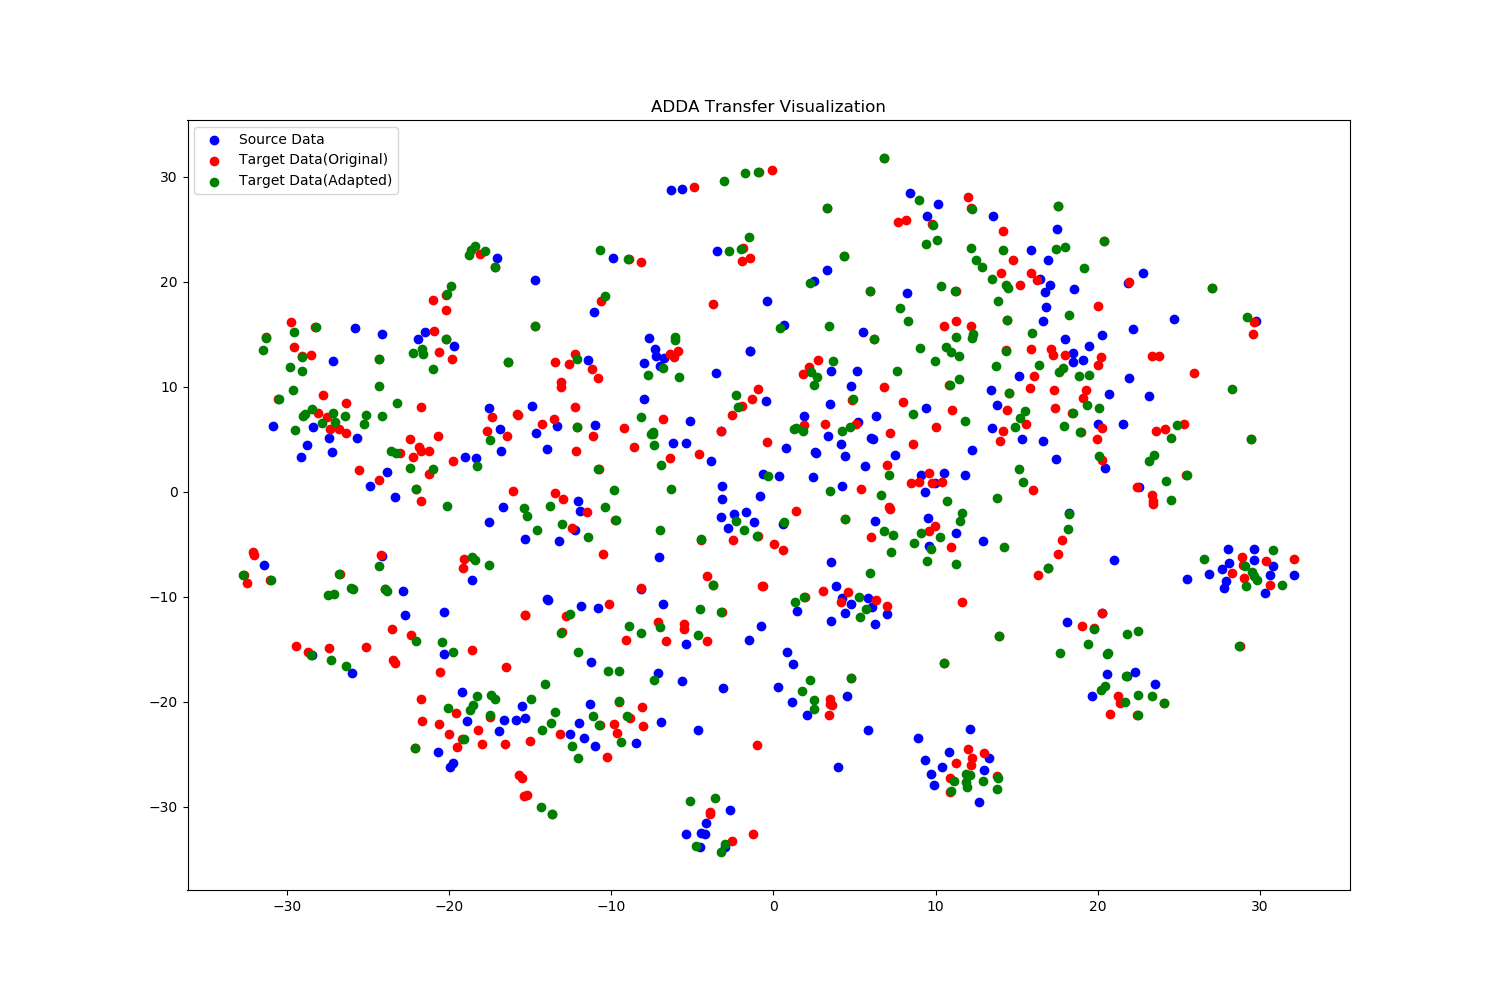
\includegraphics[width=1.6in, height=1.5in]{Ladda/std_A2R/ADDA_visual.png}
\end{minipage}%
\begin{minipage}[t]{0.26\textwidth}
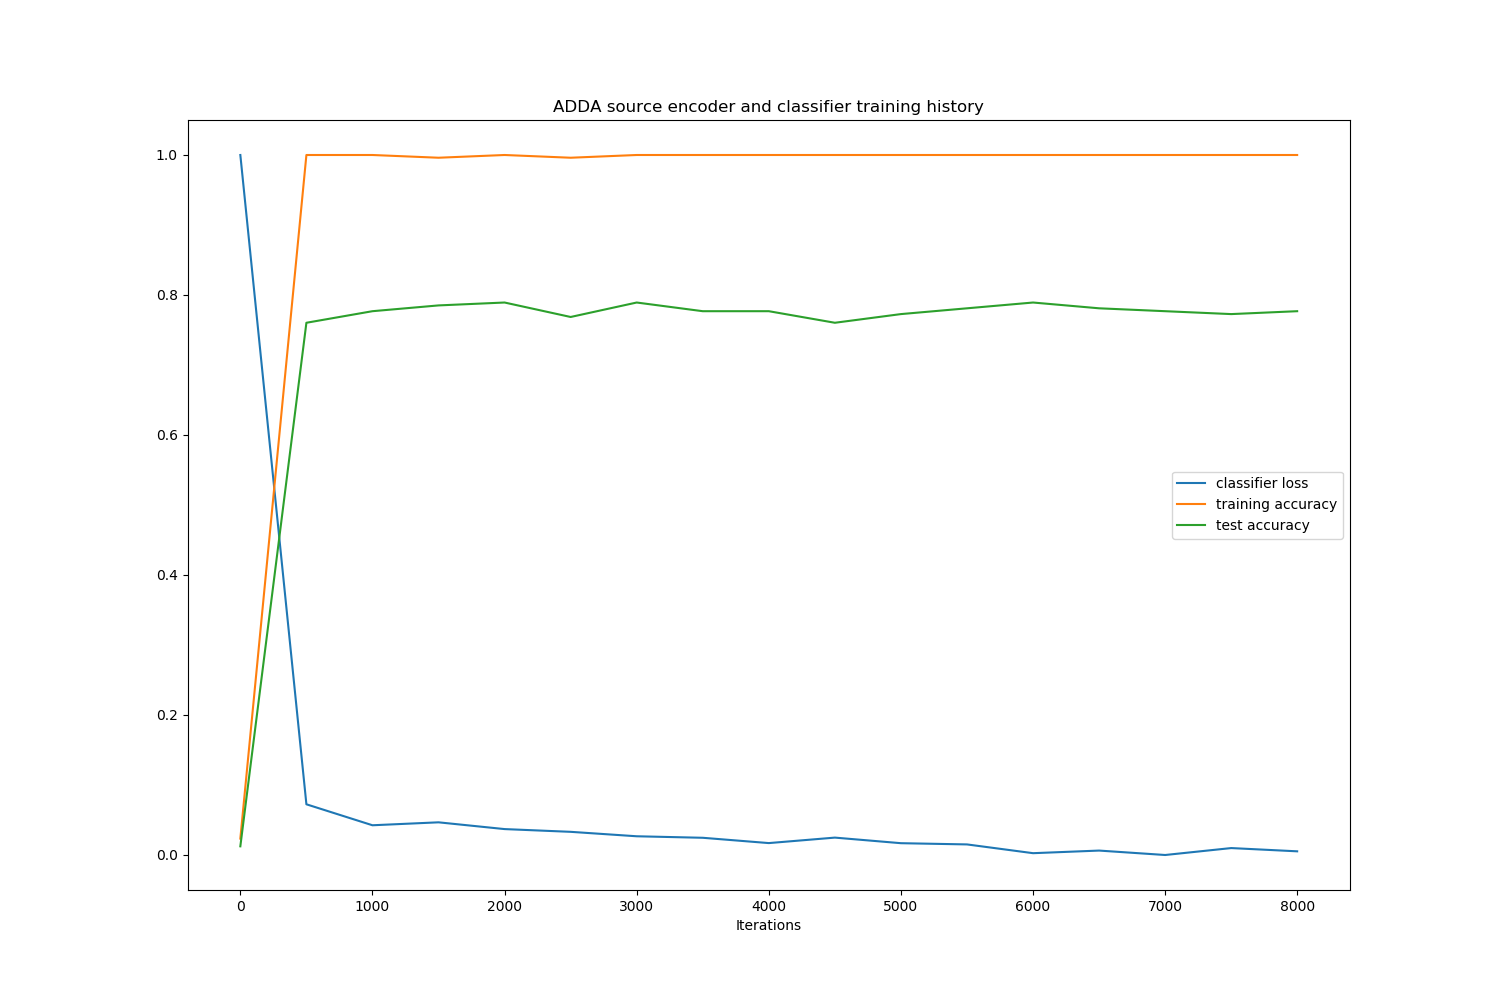
\includegraphics[width=1.6in, height=1.5in]{Ladda/std_A2R/clf.png}
\end{minipage}%
\begin{minipage}[t]{0.45\textwidth}
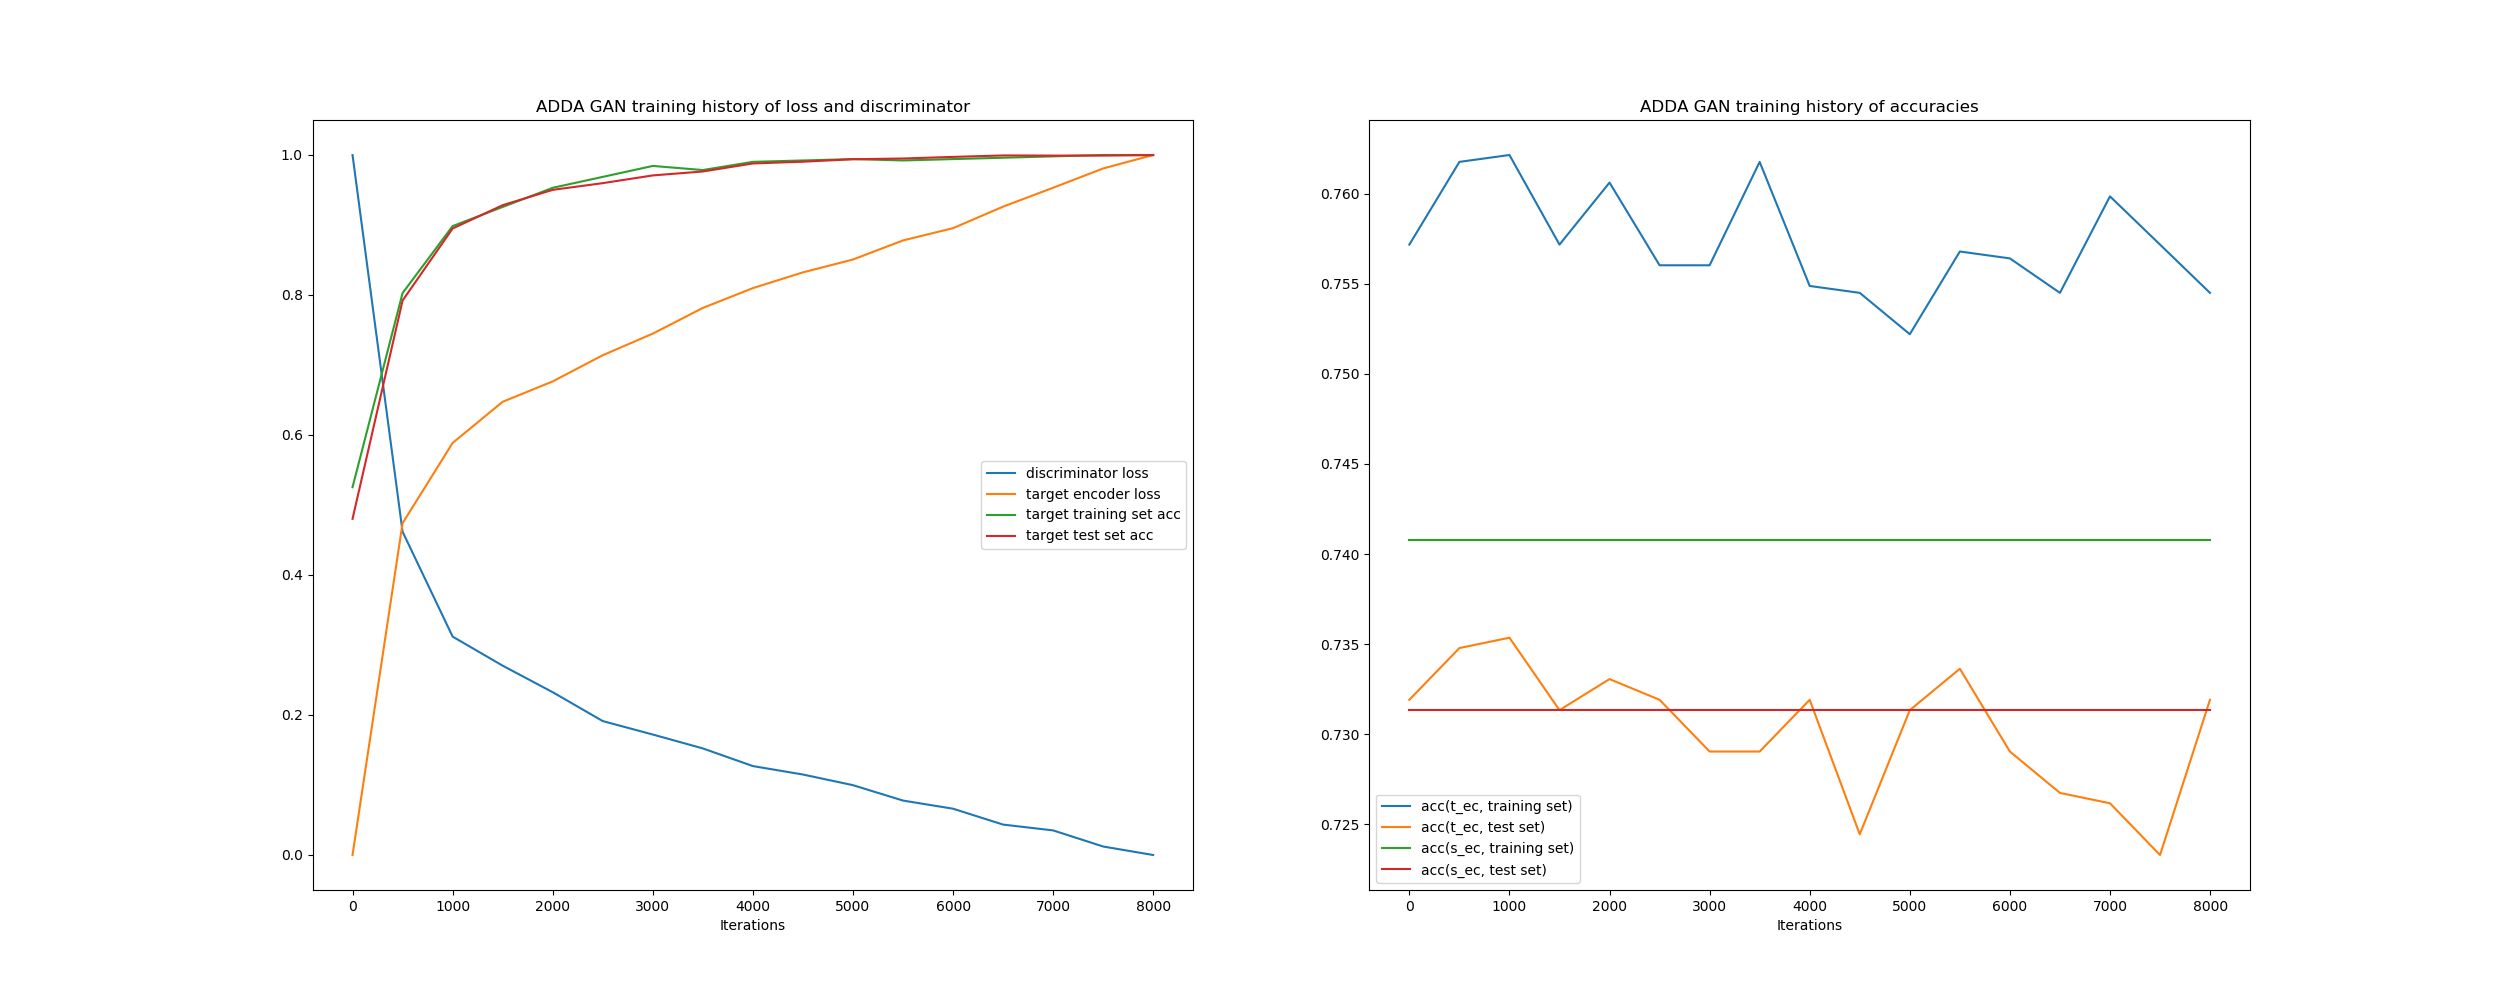
\includegraphics[width=3.5in, height=1.5in]{Ladda/std_A2R/gan.png}
\end{minipage}%
\caption{Visualization of ADDA ExA Result}\label{fig:ExA}
\end{figure*}

\begin{figure*}[htb]

\centering
\begin{minipage}[t]{0.26\textwidth}
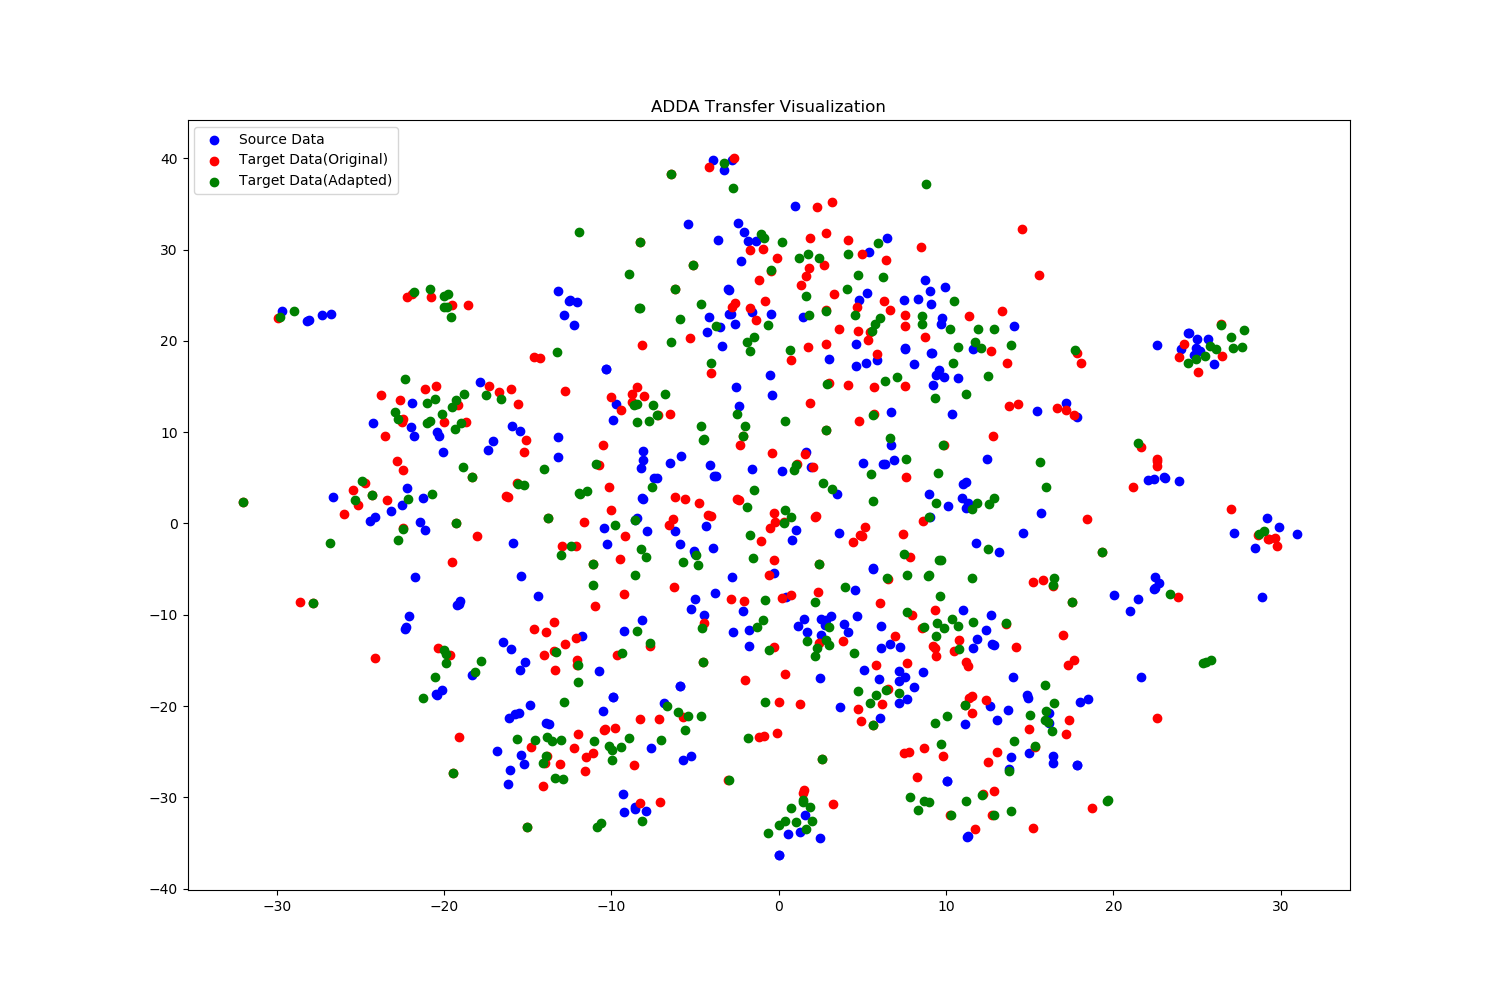
\includegraphics[width=1.6in, height=1.5in]{Ladda/std_C2R/ADDA_visual.png}
\end{minipage}%
\begin{minipage}[t]{0.26\textwidth}
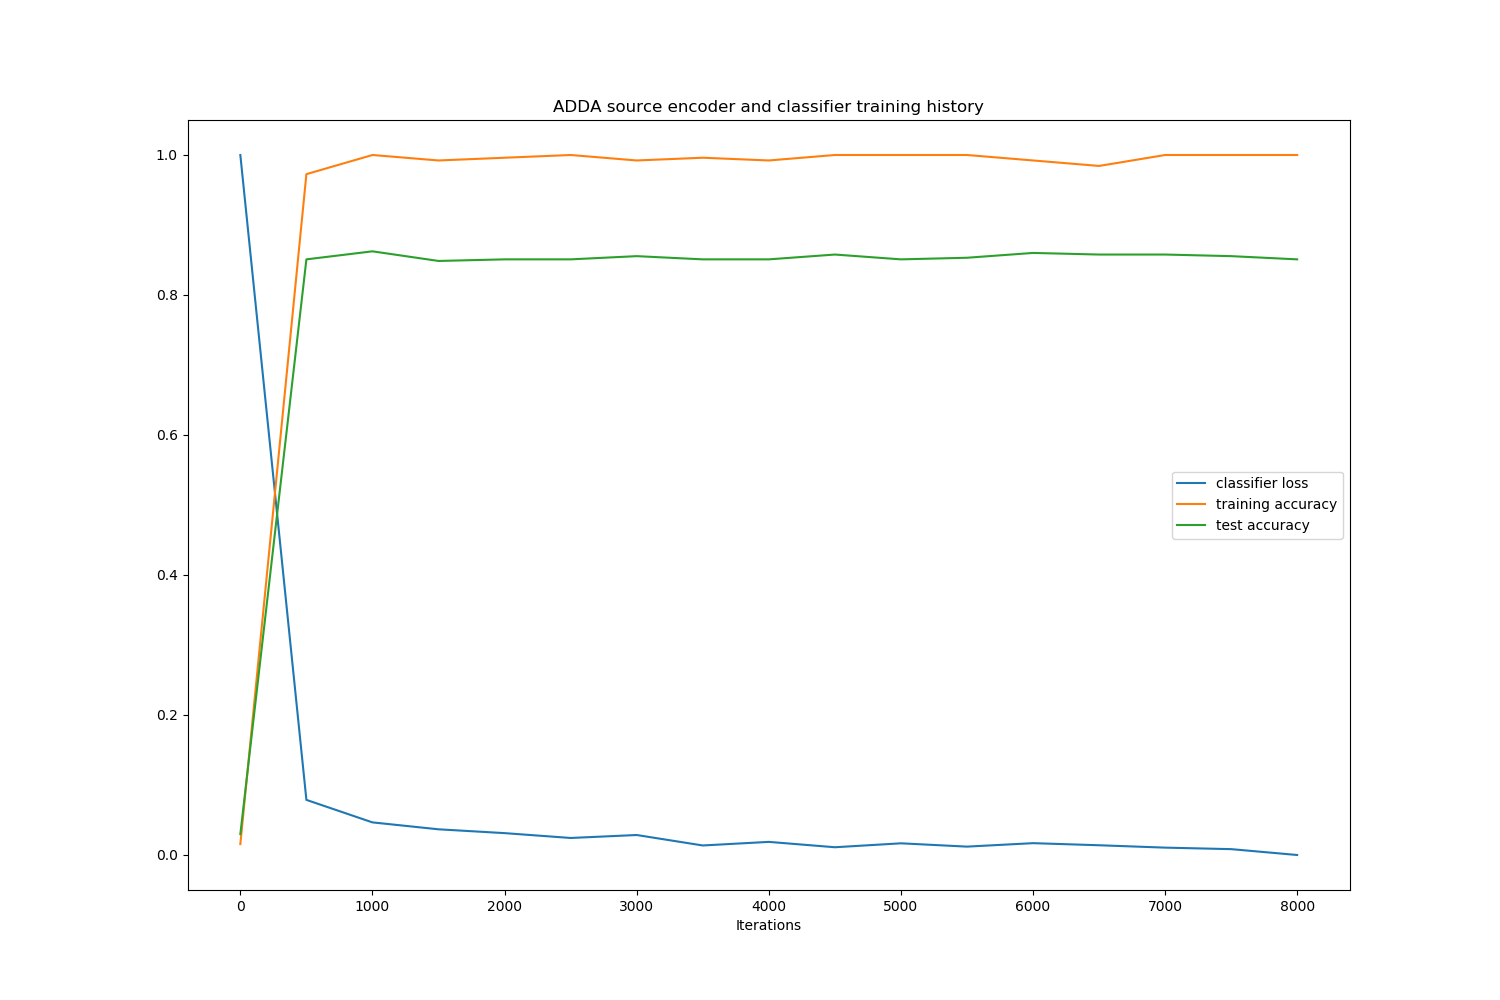
\includegraphics[width=1.6in, height=1.5in]{Ladda/std_C2R/clf.png}
\end{minipage}%
\begin{minipage}[t]{0.45\textwidth}
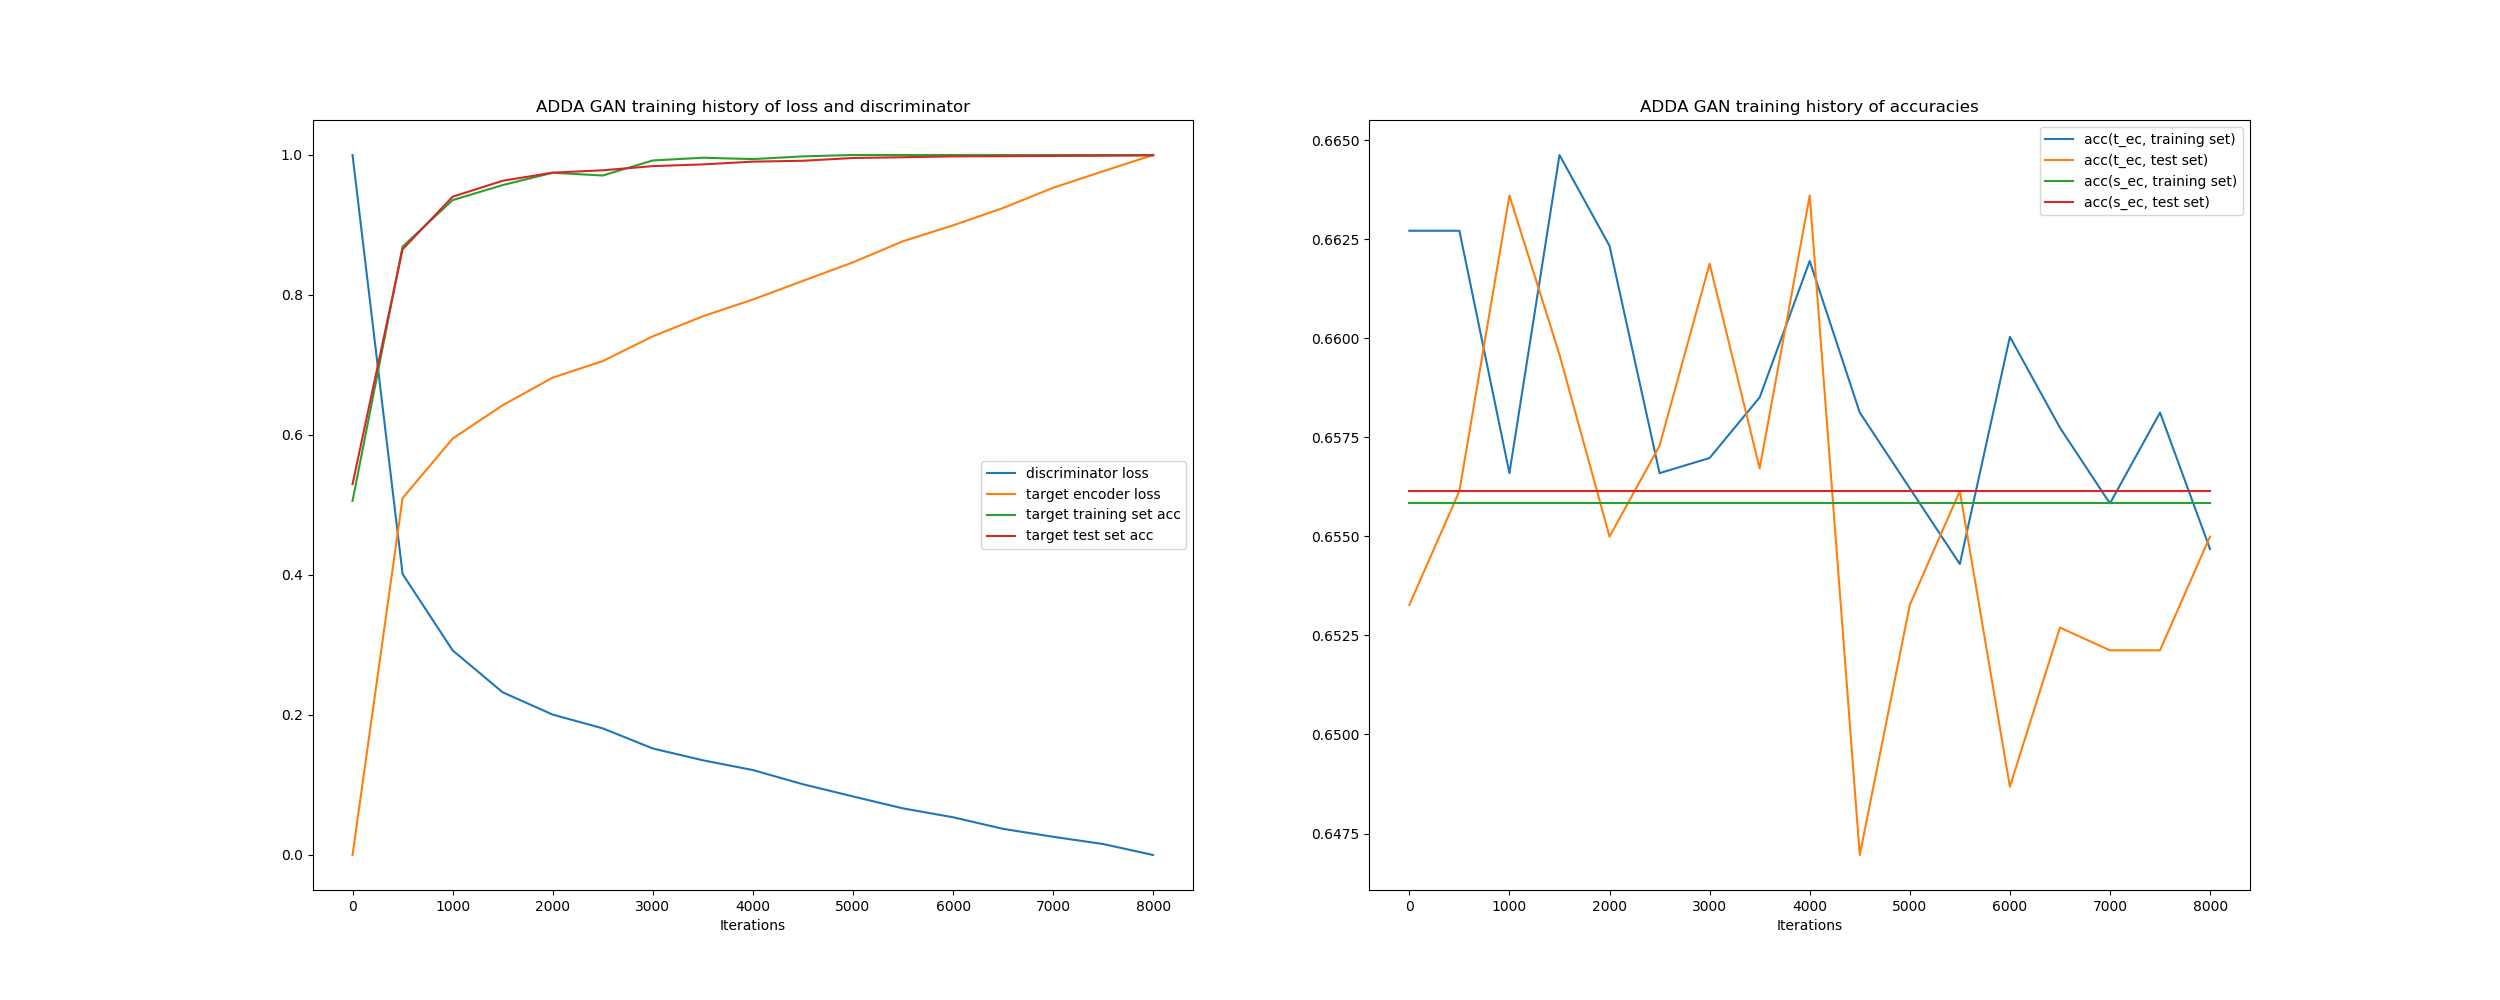
\includegraphics[width=3.5in, height=1.5in]{Ladda/std_C2R/gan.png}
\end{minipage}%
\caption{Visualization of ADDA ExC Result}\label{fig:ExC}
\end{figure*}

\begin{figure*}[htb]

\centering
\begin{minipage}[t]{0.26\textwidth}
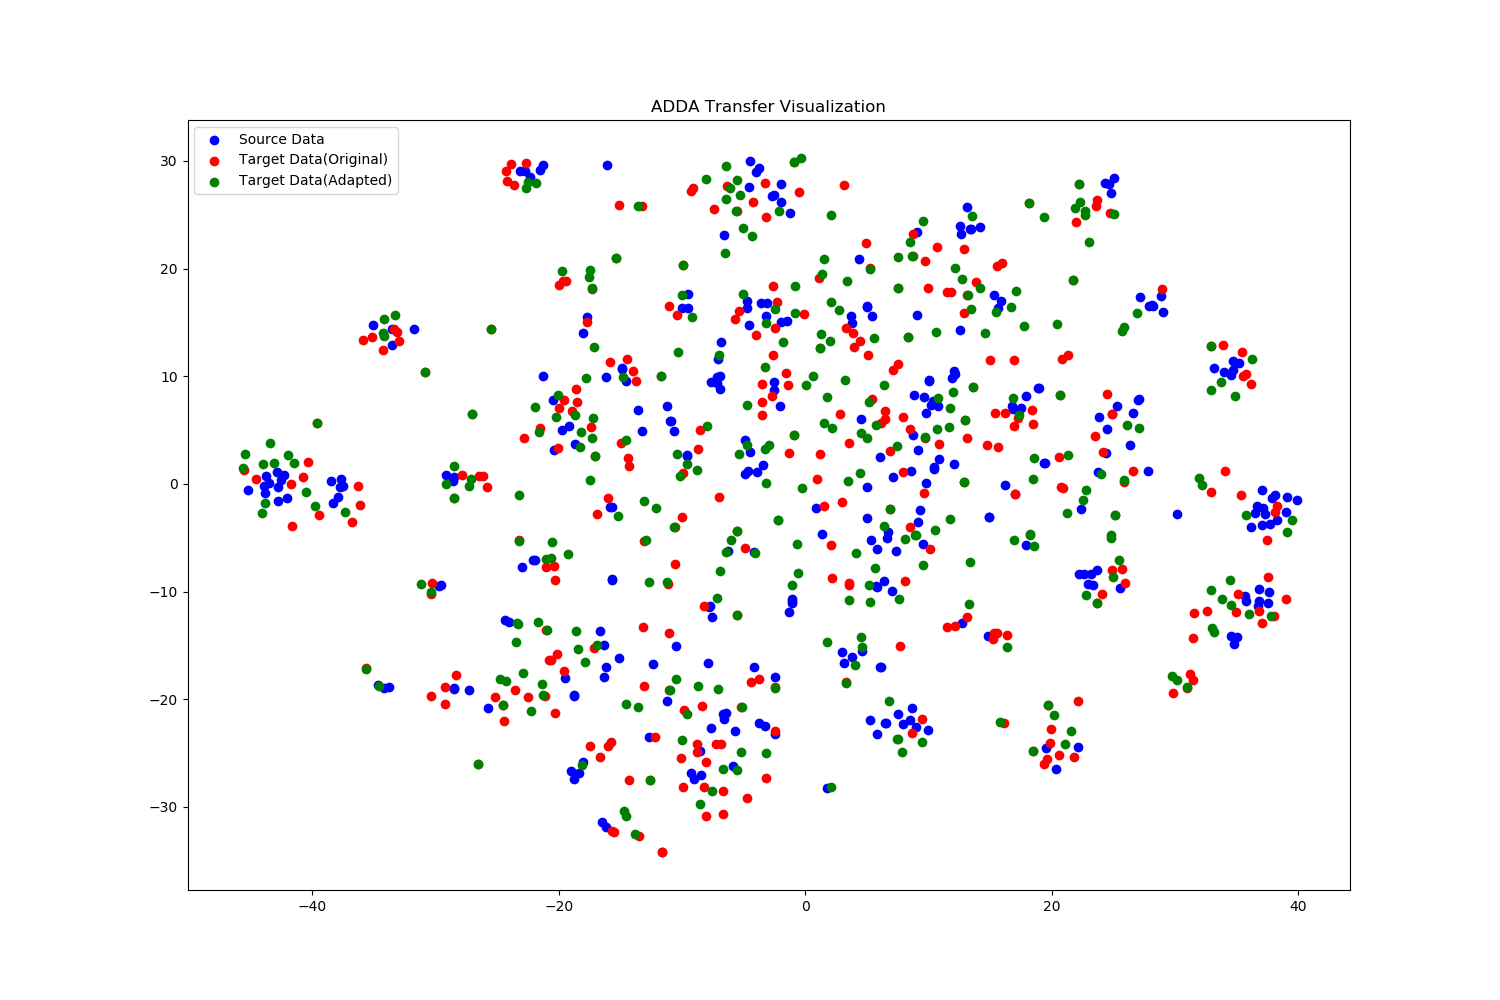
\includegraphics[width=1.6in, height=1.5in]{Ladda/std_P2R/ADDA_visual.png}
\end{minipage}%
\begin{minipage}[t]{0.26\textwidth}
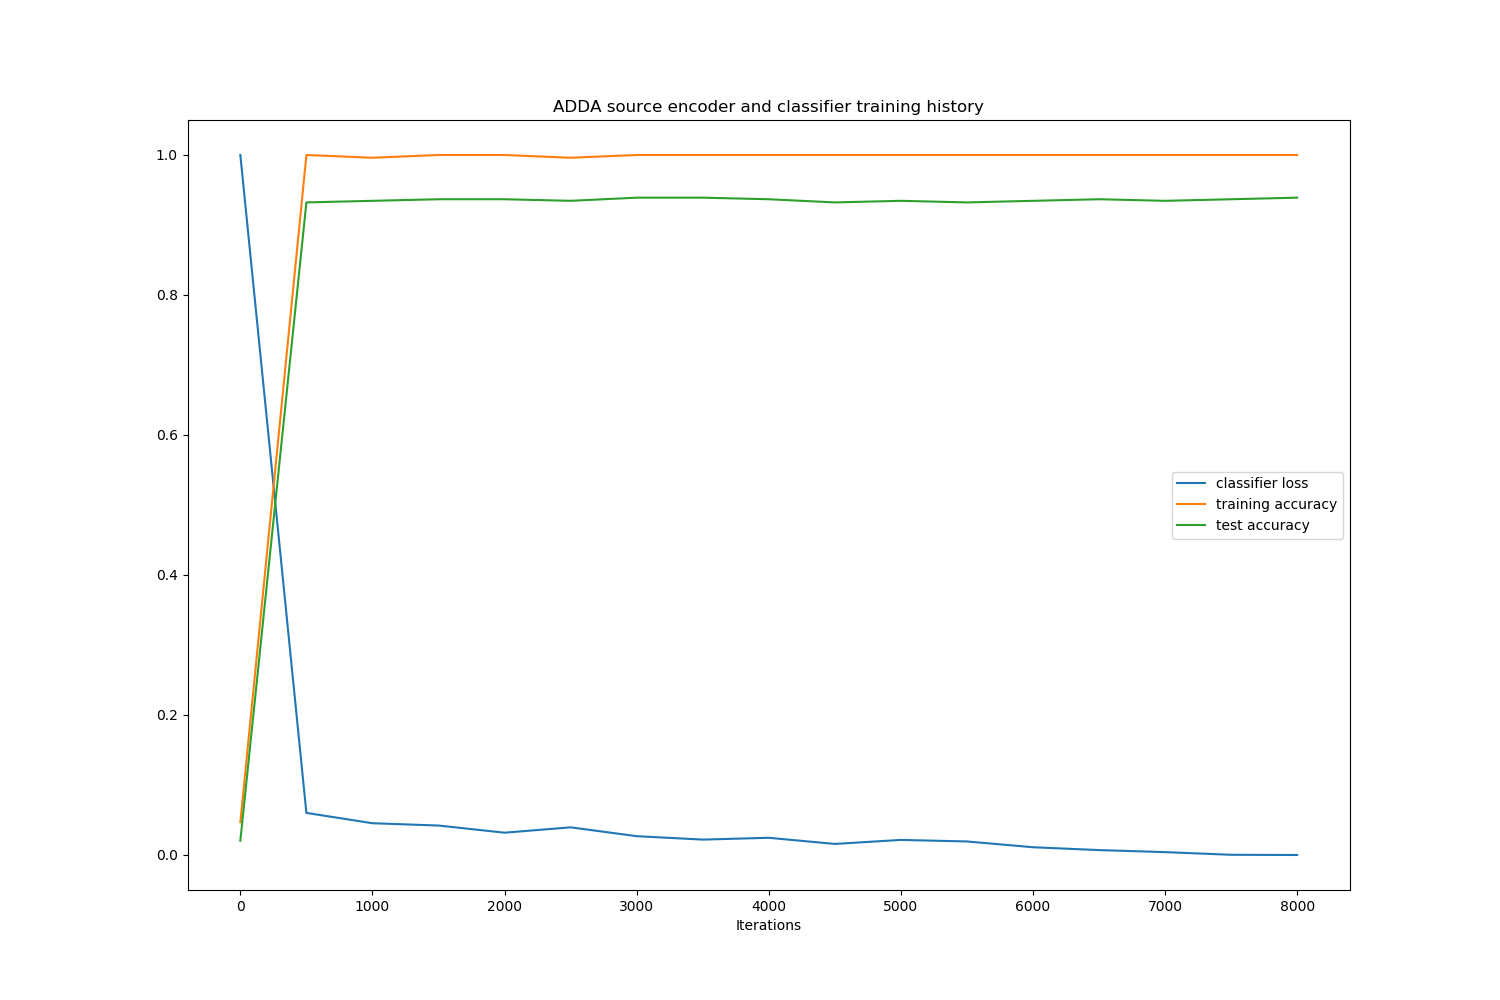
\includegraphics[width=1.6in, height=1.5in]{Ladda/std_P2R/clf.png}
\end{minipage}%
\begin{minipage}[t]{0.45\textwidth}
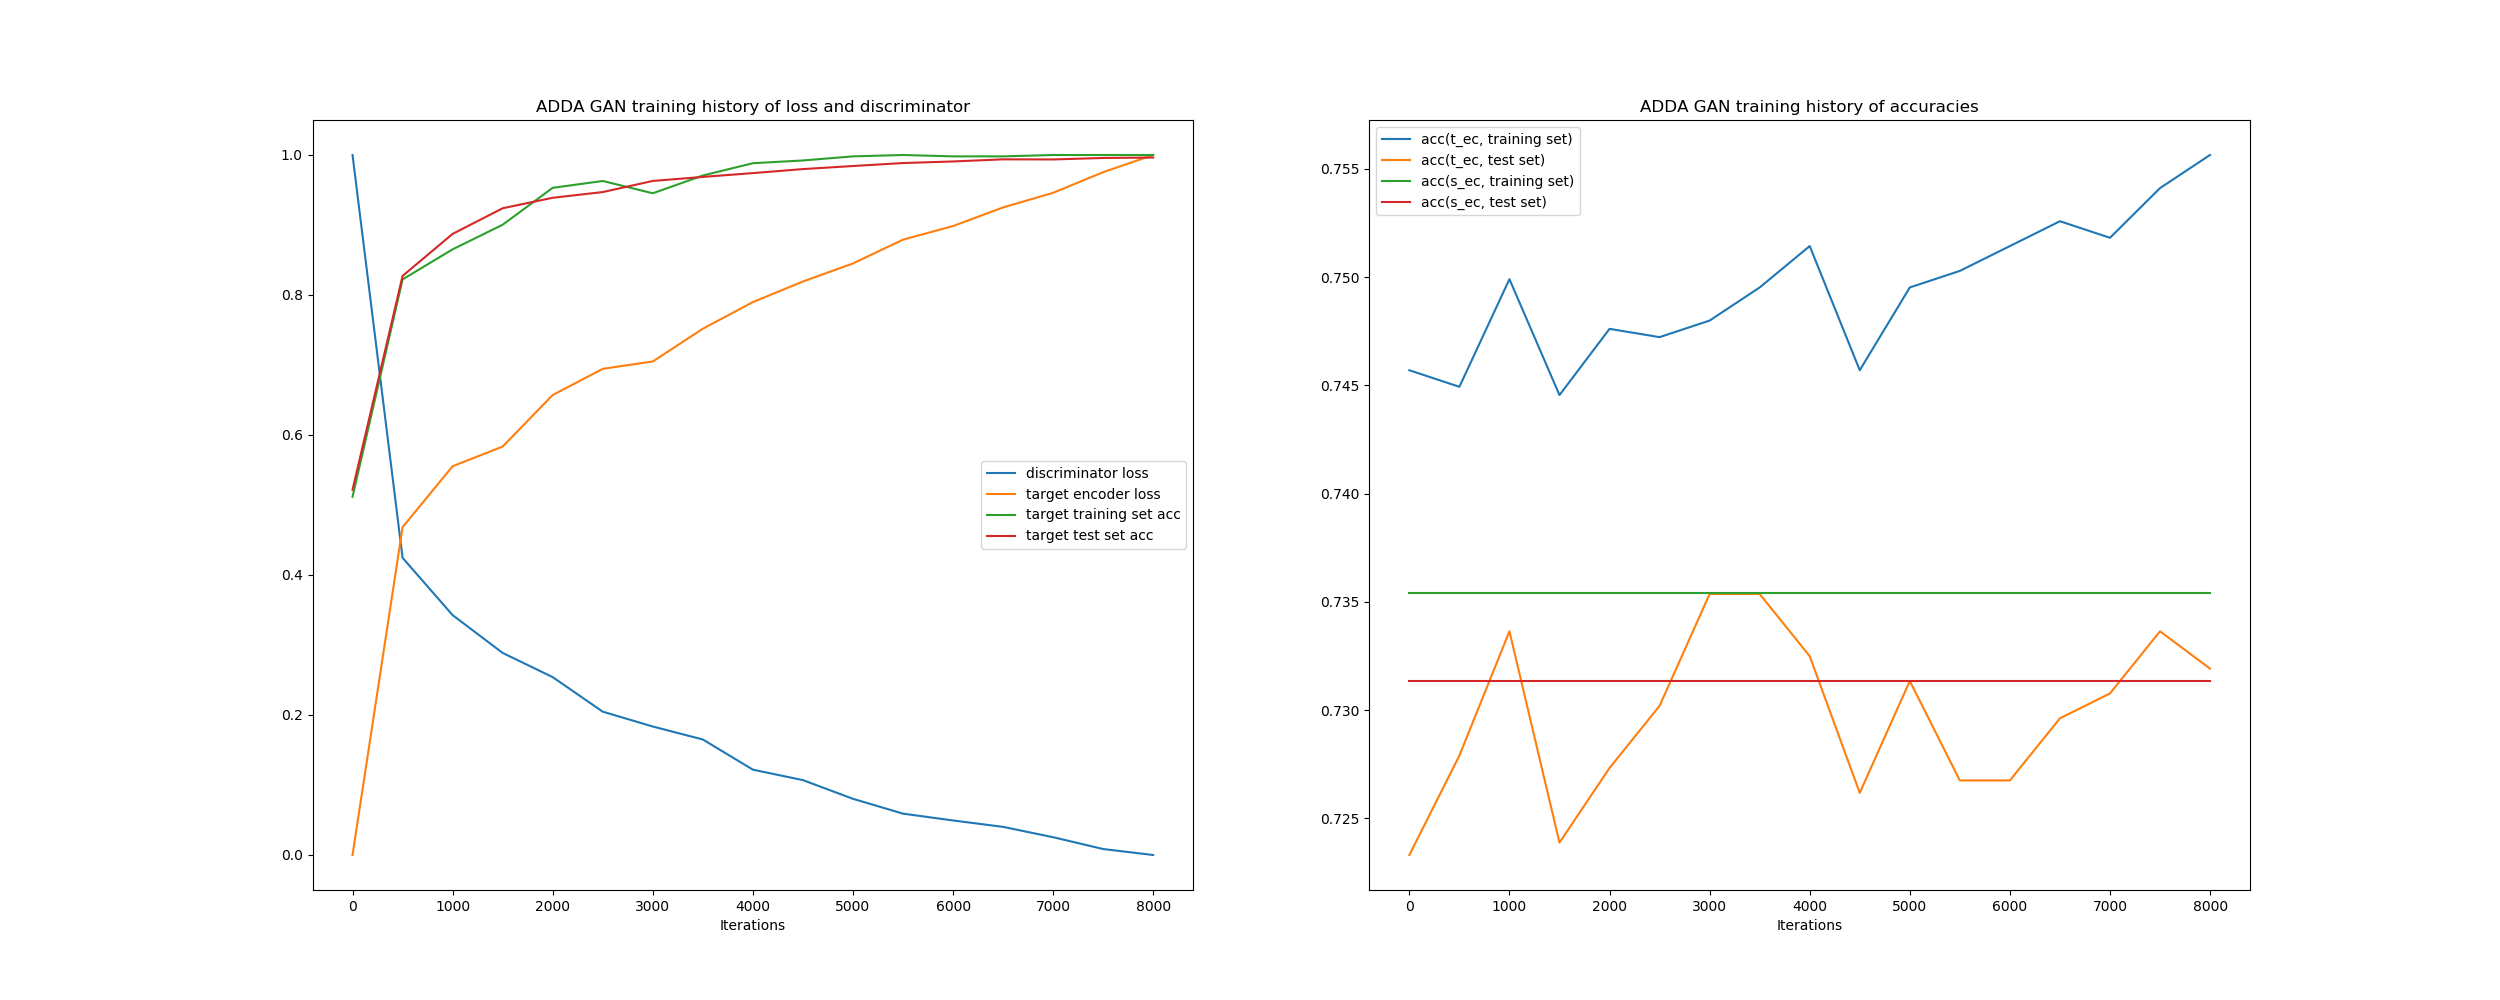
\includegraphics[width=3.5in, height=1.5in]{Ladda/std_P2R/gan.png}
\end{minipage}%
\caption{Visualization of ADDA ExP Result}\label{fig:ExP}
\end{figure*}


\subsection{DANN Experiments}
We present three experiments using DANN method. Because of time issue, we did not design DANN experiments that sophisticatedly, but we learned a lot from ADDA experiments. Common hyper-parameters are listed in table \ref{tab:SymDANN}. Tricks of L2 normalization and neuron dropout are not used in the experiments because these tricks did not perform that well as expected in the previous experiments of DANN. And we use sigmoid function for activation of hidden layers. Also, a softmax layer is added after the output layer before calculating cross entropy. Batch normalization is not applied in DANN experiments. DANN networks we designed are much simpler and more light-weighted. Learning rate, $l_r$, of both two stages anneals according to the formula: $l_r= \frac{0.00004}{ (1.0 + \frac{1.0 \times i}{I})^{0.75}}$, where $i$ is the current iteration. Primitive of the formula was proposed in Yaroslav Ganin, et al.'s work. We just adjust some factors according to our preliminary experiments.
 \begin{table}[h]
	\centering
	\caption{Hyper-parameters of DANN}
	\label{tab:SymDANN}
	\begin{tabular}{ccc}
		\hline
		Symbol & Value & Description \\
		\hline
		\hline
        $K$ & $65$ & Number of classes \\
		$b$ & $256$ & Batch size \\
		$l_e$ & ${2048,1024}$ & Layers of $M$ \\
		$l_c$ & ${256,K}$ & Layers of $C$, connected from o$M$  \\
		$l_d$ & ${512,512,2}$ & Layers of $D$, connected from $M$ \\
        $p_k$ & $0.0$ & Dropout probability of a neuron. \\
        $r^{tr}_{s}$ & $0.75$ & Ratio of $X_s$ used as training set.\\
        $r^{tr}_{t}$ & $0.75$ & Ratio of $X_t$ used as training set.  \\
        $I$ & $8000$ & Total iterations of first two training stages.   \\
		\hline
	\end{tabular}
\end{table}


 \begin{table*}[h]
	\centering
	\caption{Different Configurations And Resulted Performances of DANN Experiments}
	\label{tab:ConfigDANN}
	\begin{tabular}{ccccccc}
		\hline
		Sym & Src & $Ac(M_s(X^{te}_s))^*$ & $Ac(M_s(X^{te}_t))^*$ & $Ac(M_t(X^{tr}_t))^*$ & $Ac(M_t(X^{te}_t))^*$ & g\\
		\hline
		\hline
		$Ex_A$ &  Art & 0.8020 & 0.7172 & 0.7488 & 0.7301 & 0.0129\\
		$Ex_C$ &  Clipart & 0.8671 & 0.6501 & 0.6683 & 0.6547 & 0.0046\\
		$Ex_P$ &  Product &  0.9596 & 0.7328 & 0.7411 & 0.7392 & 0.0064\\
		\hline
	\end{tabular}
\end{table*}
We first present an overview of all of the three DANN experiments in table \ref{tab:ConfigDANN}. Different from ADDA model, we have only one encoder $M$ in DANN. $M$ is trained with $(X_s, Y_x)$ in the first stage and then trained to adapt target domain in the second stage. Thus, to maintain consistency of our symbols, we use $M_s$ to represent the encoder after the first-stage training and $M_t$ to represent the encoder after the second-stage training.

Compared with the results of ADDA shown in the last three rows of table \ref{tab:ConfigADDA}, except the first-stage trained classification accuracies towards source test set, $Ac(M_s(X^{te}_s))^*$, show better performances, the other three indicators fall. The classifier works better with source domain dataset after pre-training but doesn't show such improvement when it comes to classify adapted target domain data.

Figures \ref{fig:ExA2}, \ref{fig:ExC2}, \ref{fig:ExP2} shows visualization of the three DANN experiments. The are four subfigures in each figure. The first two subfigures illustrate visualization of encoded source and target data distribution before($M_s(X^{te}_s)$, $M_s(X^{te}_t)$) and after($M_t(X^{te}_s)$, $M_t(X^{te}_t)$) domain adaptation. The third subfigure shows training history of the classifier $C$ in the pre-train stage. We name feature encoder in this stage $M_s$. Legends of "source accuracy(test)" and "source accuracy(train)" represent $Ac(M_s(X^{te}_s))$ and $Ac(M_s(X^{tr}_s))$ respectively. The fourth figure shows training history of the adversarial adaptation stage. Recall that discriminator $D$ and feature encoder $M$ are trained in this stage, and we name feature encoder in this stage $M_t$.  Legends of "source accuracy(test)", "target accuracy(test)", "source accuracy(train)" and "target accuracy(train)" represent $Ac(M_t(X^{te}_s))$, $Ac(M_t(X^{te}_t))$, $Ac(M_t(X^{tr}_s))$ and $Ac(M_t(X^{tr}_t))$ respectively.

Unlike ADDA, the power of $D$ doesn't improve so smoothly. We think it is because we are not minimizing $L_C$ and $L_D$ respectively but minimizing $L_{da} = L_C+L_D$. We want to keep a good performance of classifier $C$ the same time when trying to adjust $M$ to adapt the target domain data.

\begin{figure*}[htb]
\centering
\begin{minipage}[t]{0.2\textwidth}
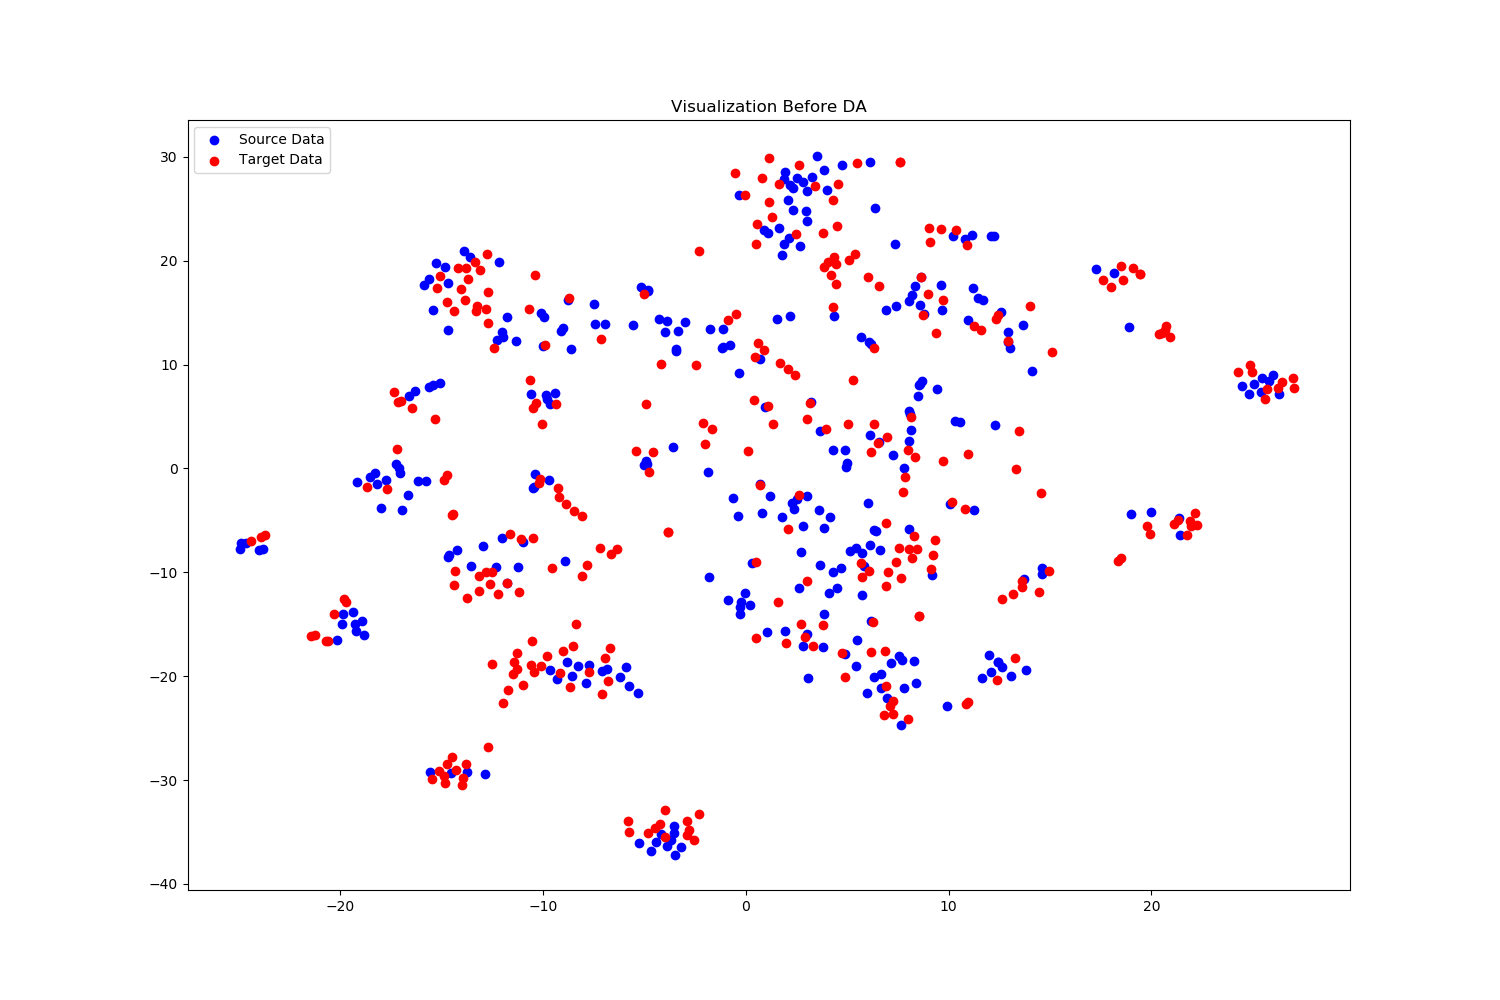
\includegraphics[width=1.5in, height=1.5in]{Ldann/std_A2R/before.png}
\end{minipage}%
\begin{minipage}[t]{0.2\textwidth}
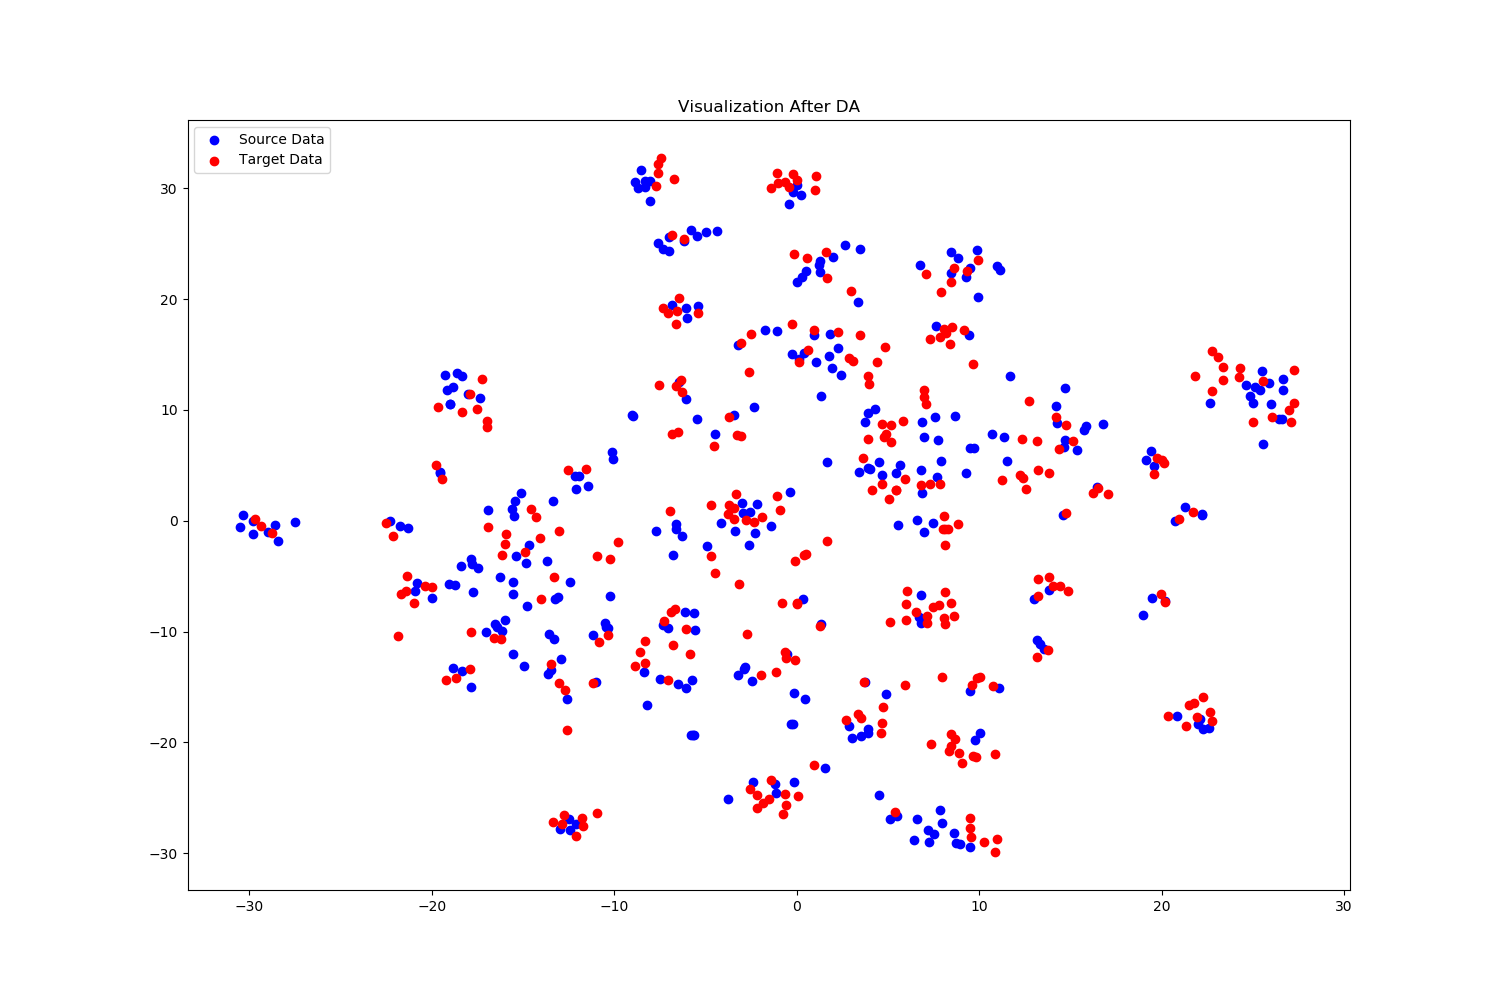
\includegraphics[width=1.5in, height=1.5in]{Ldann/std_A2R/after.png}
\end{minipage}%
\begin{minipage}[t]{0.45\textwidth}
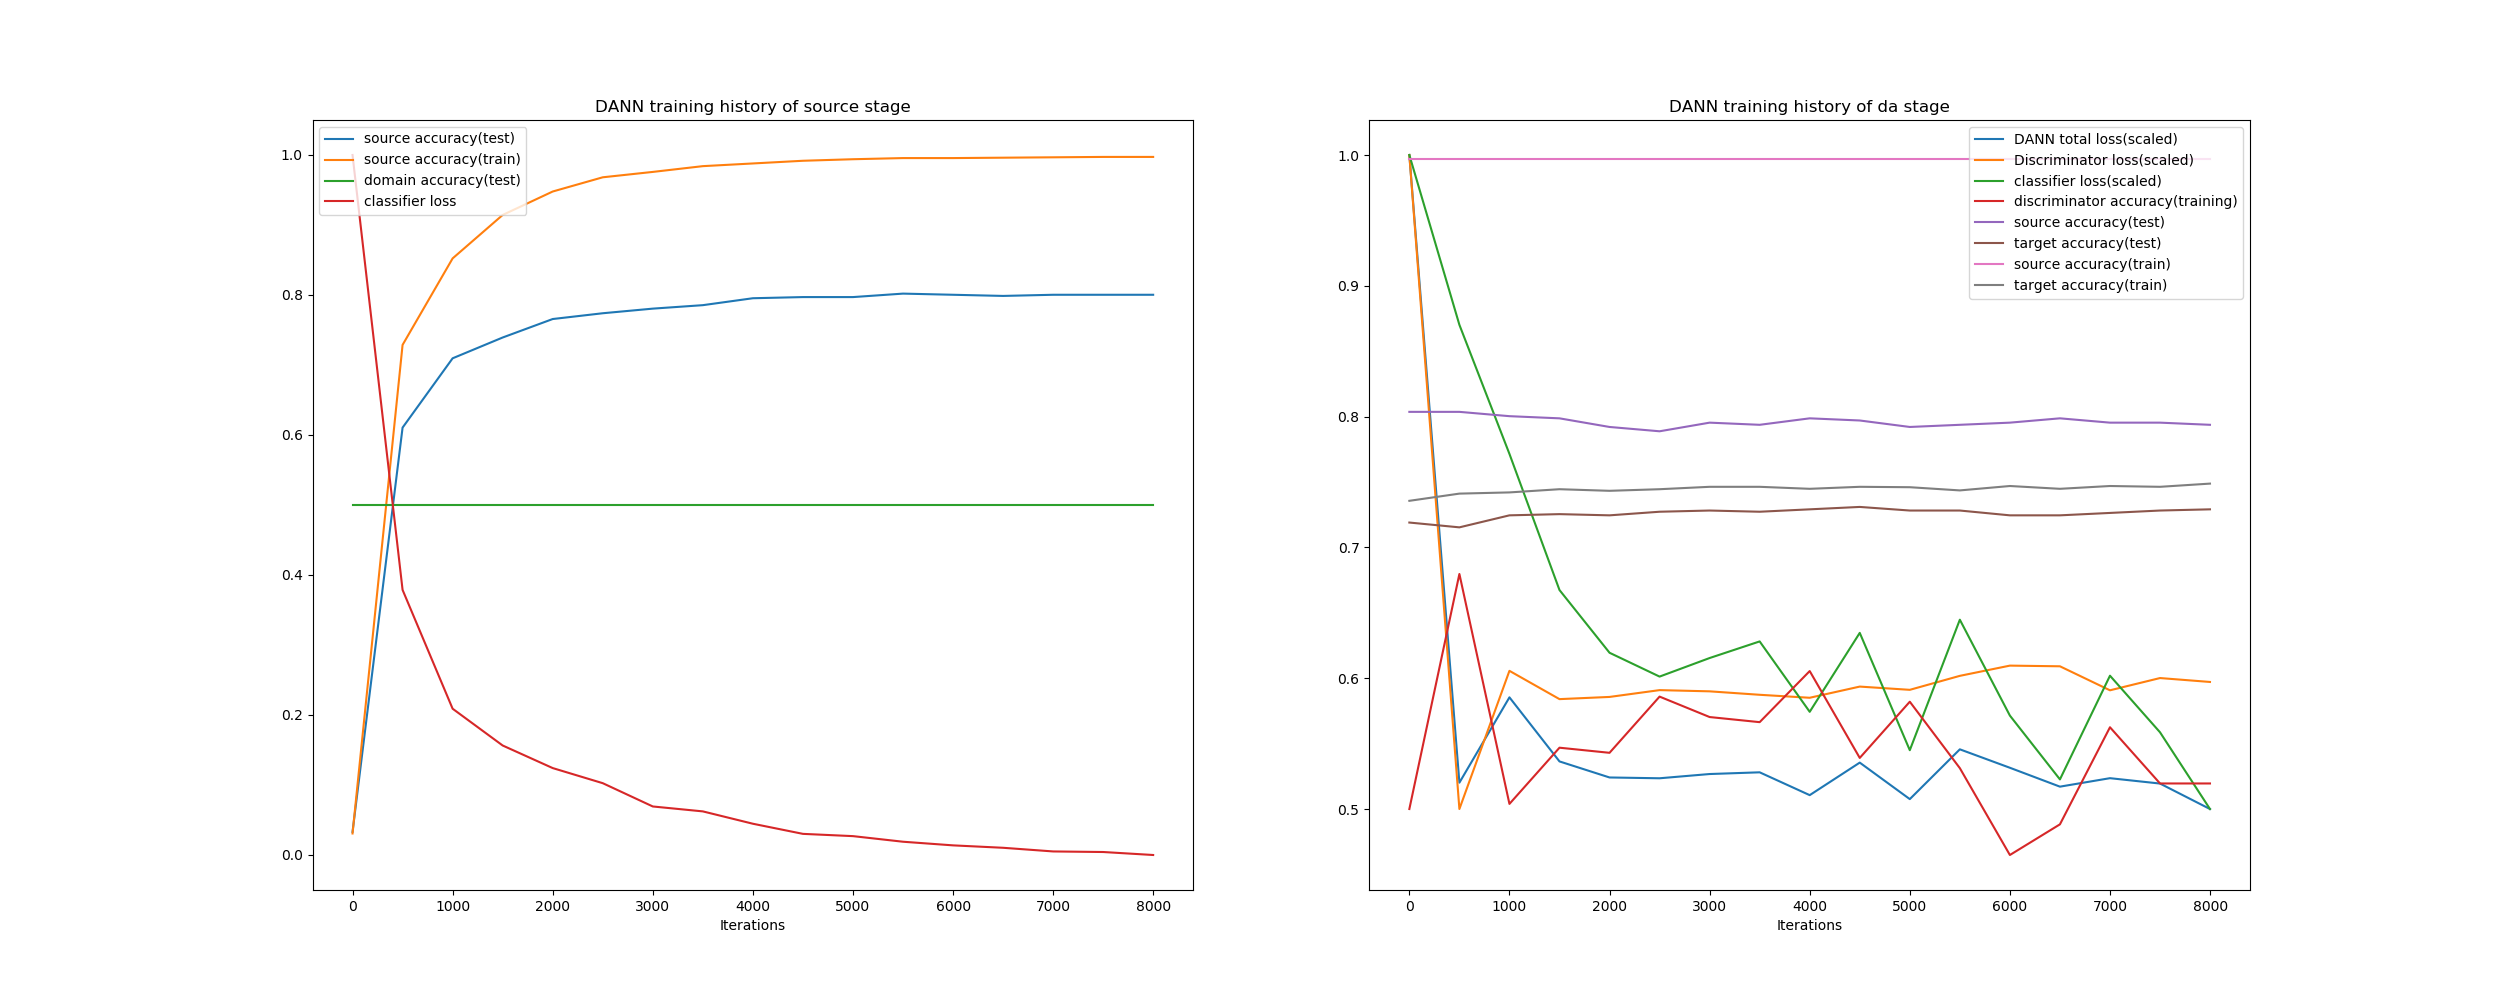
\includegraphics[width=3.5in, height=1.5in]{Ldann/std_A2R/dann.png}
\end{minipage}%
\caption{Visualization of DANN ExA Result}\label{fig:ExA2}
\end{figure*}

\begin{figure*}[htb]
\centering
\begin{minipage}[t]{0.2\textwidth}
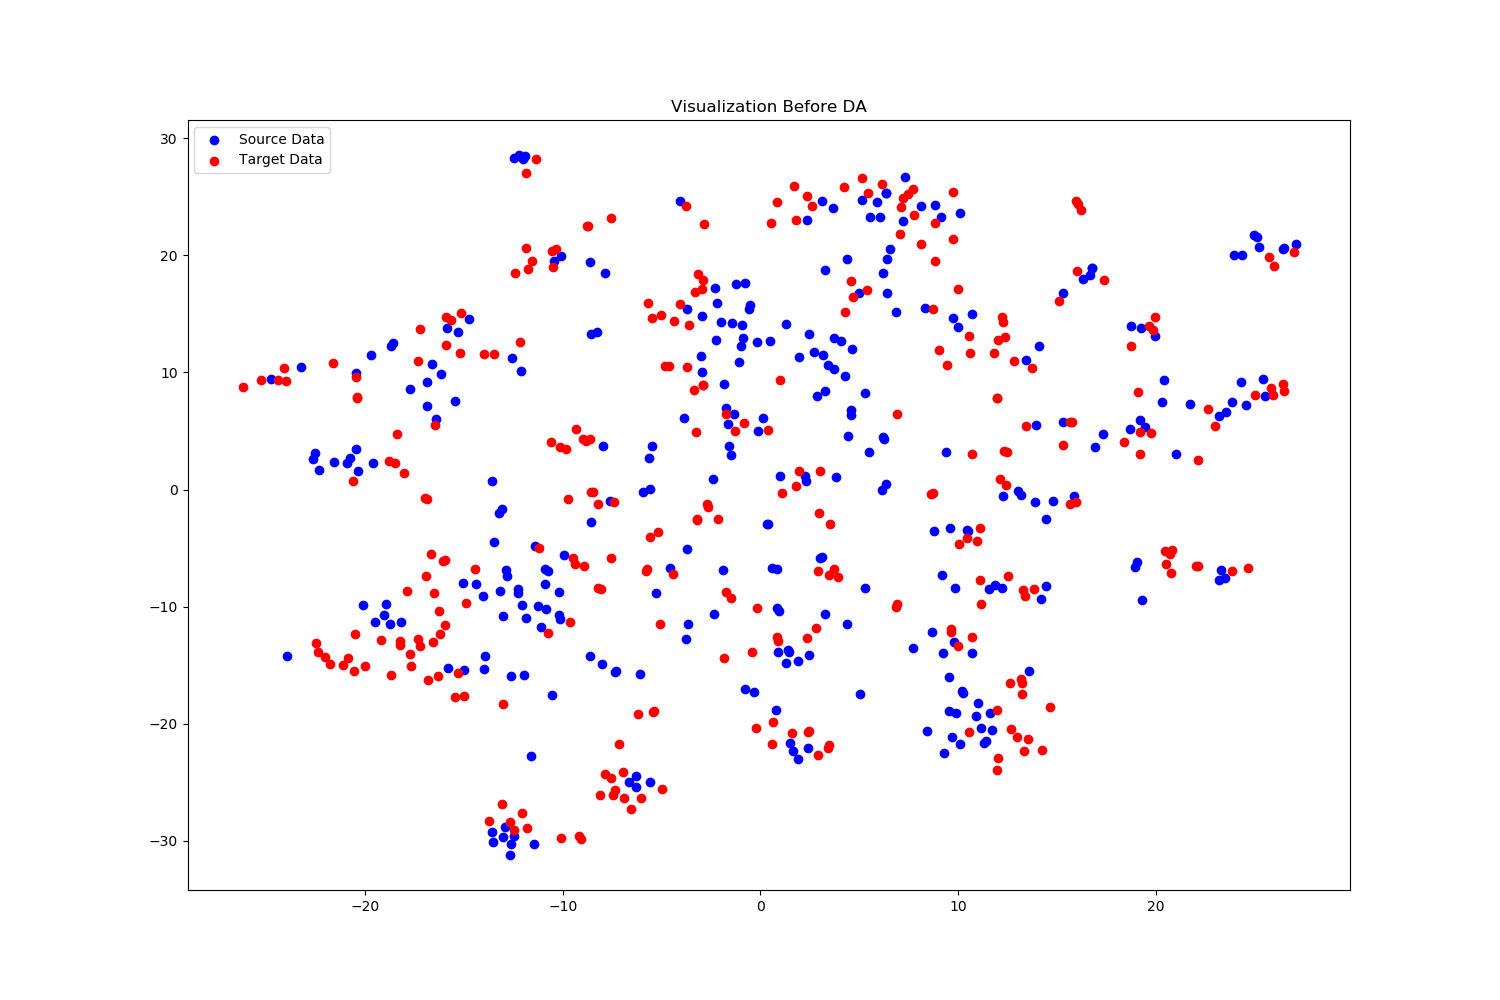
\includegraphics[width=1.5in, height=1.5in]{Ldann/std_C2R/before.png}
\end{minipage}%
\begin{minipage}[t]{0.2\textwidth}
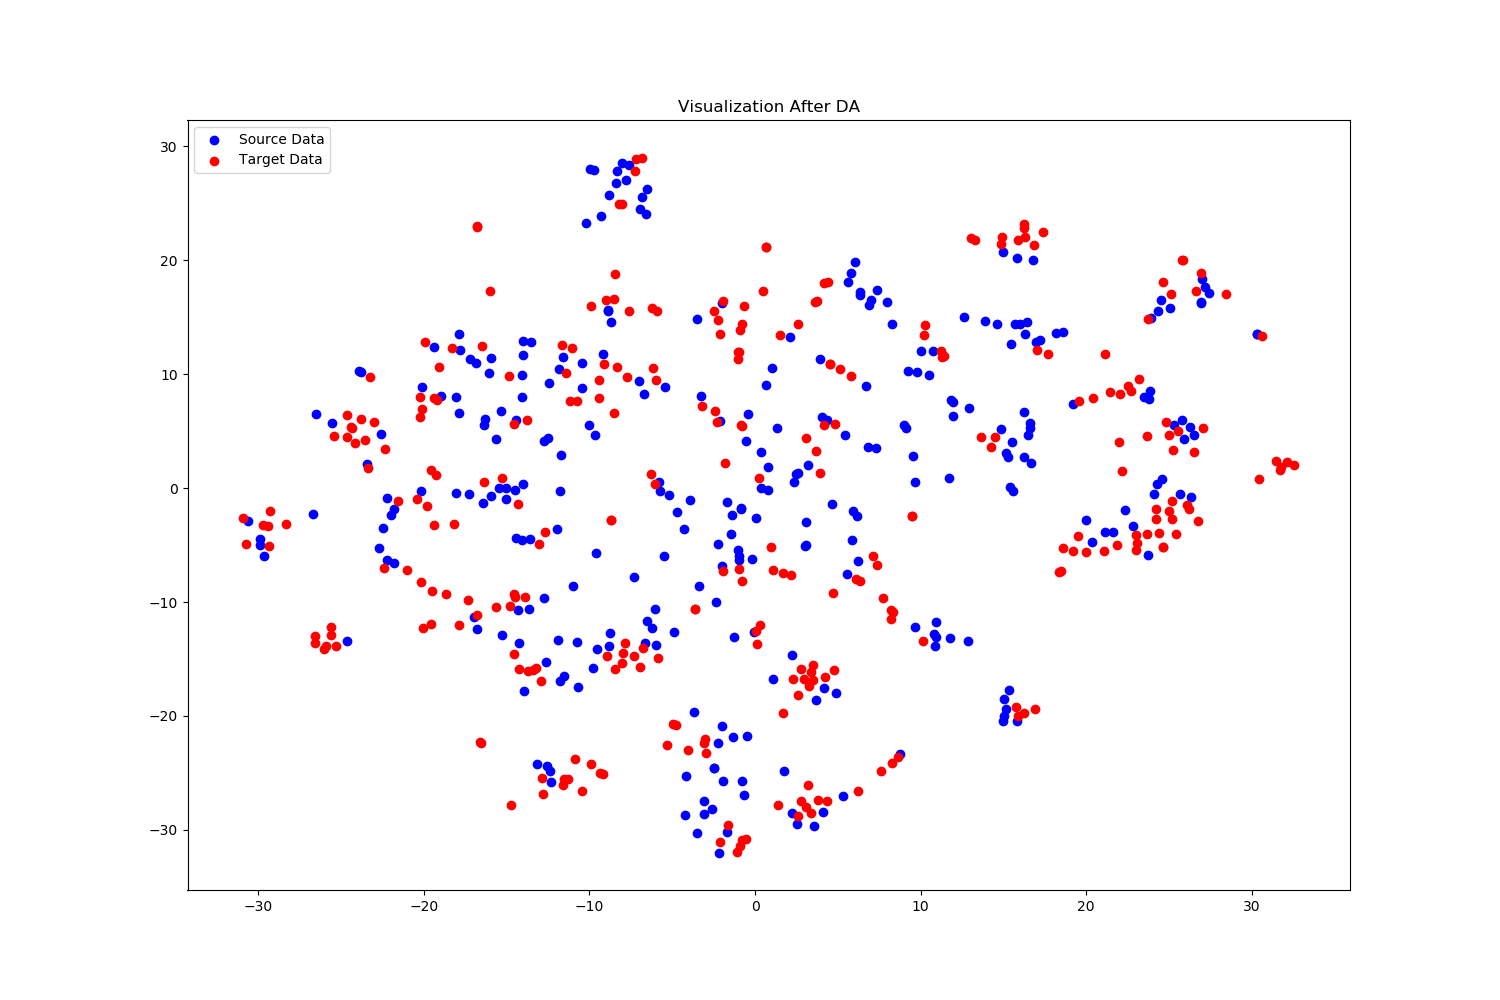
\includegraphics[width=1.5in, height=1.5in]{Ldann/std_C2R/after.png}
\end{minipage}%
\begin{minipage}[t]{0.45\textwidth}
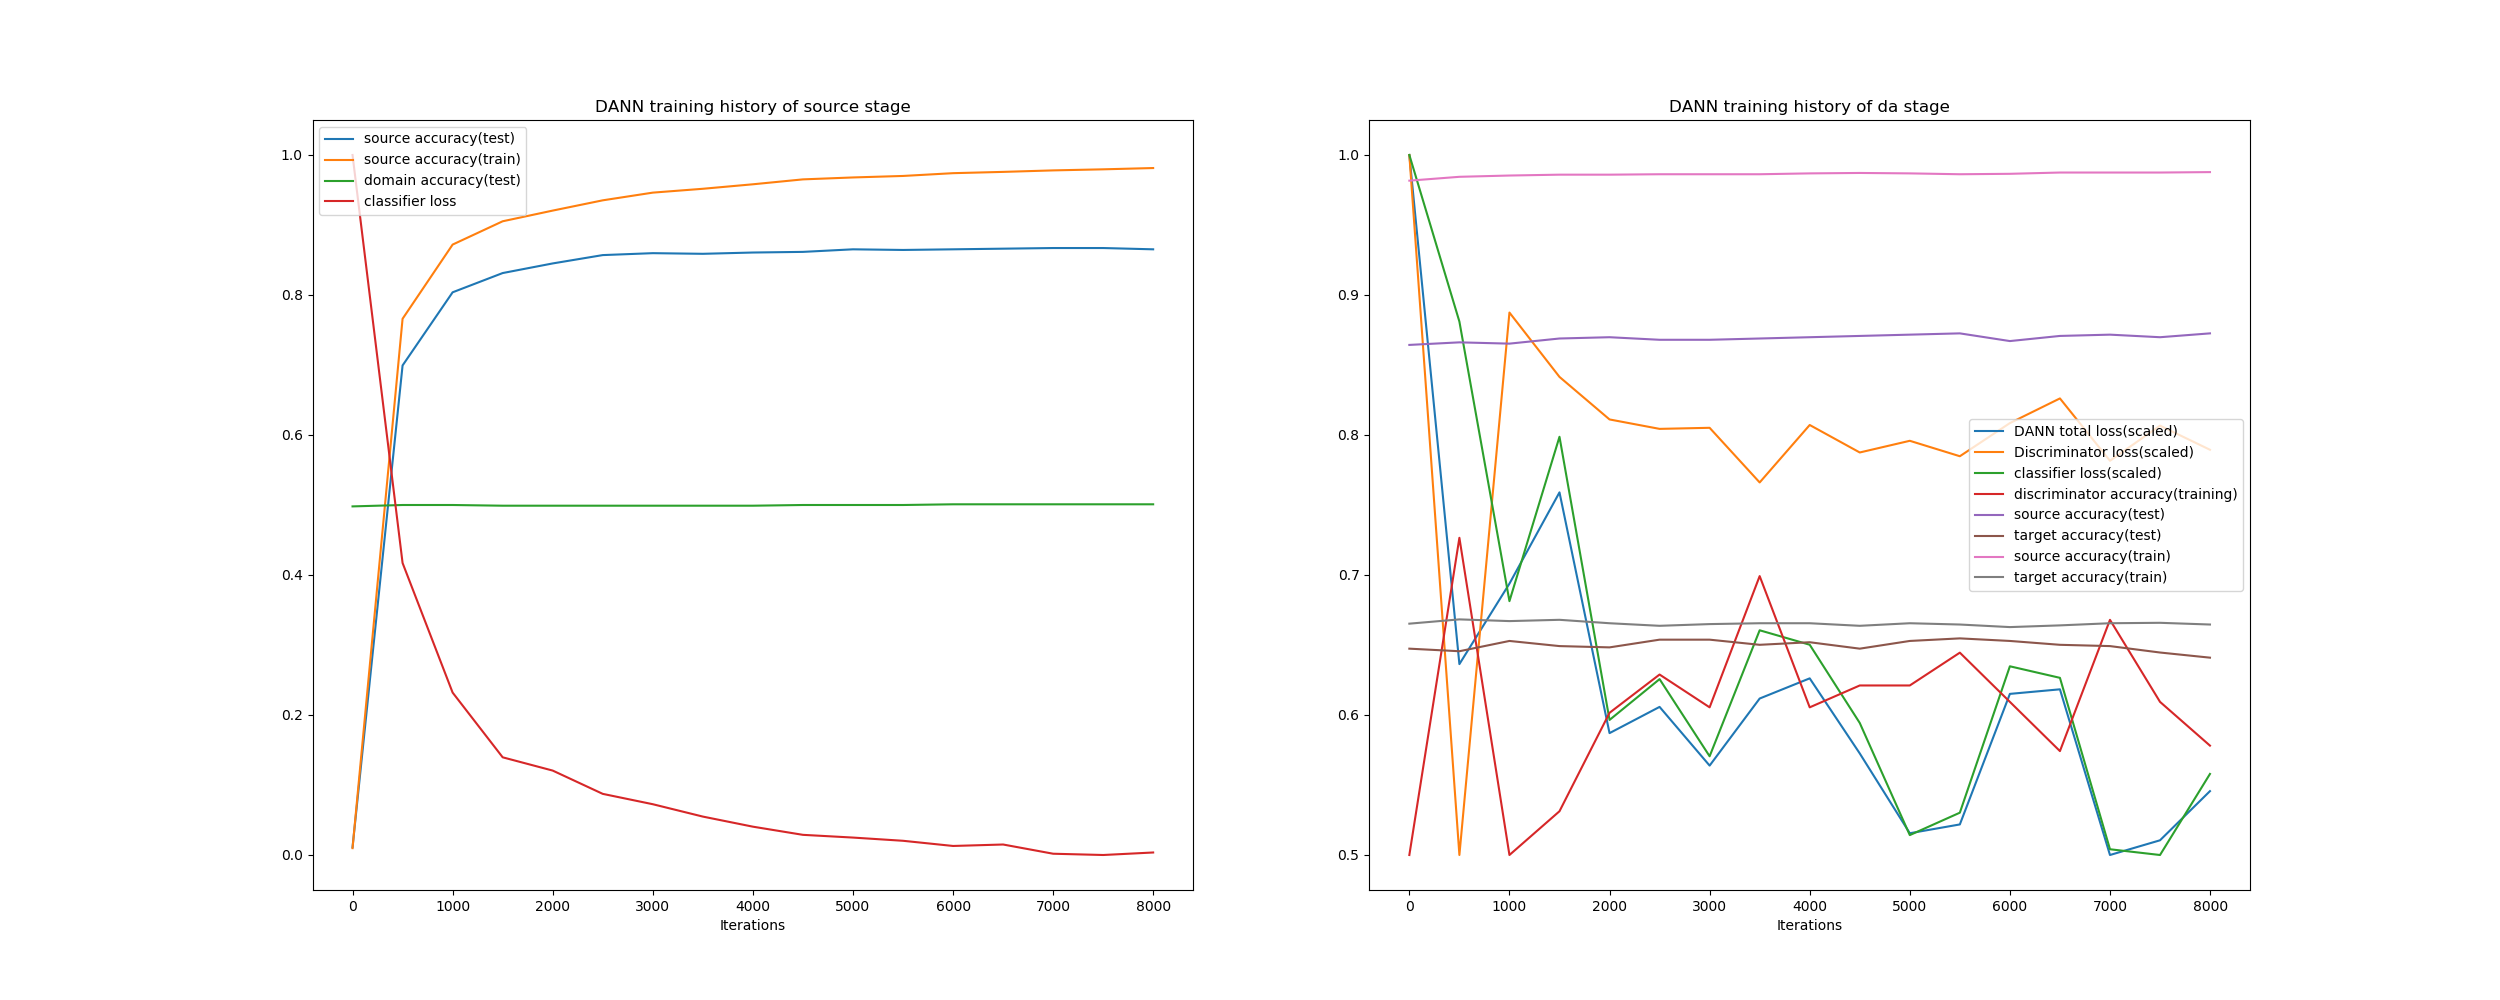
\includegraphics[width=3.5in, height=1.5in]{Ldann/std_C2R/dann.png}
\end{minipage}%
\caption{Visualization of DANN ExC Result}\label{fig:ExC2}
\end{figure*}

\begin{figure*}[htb]
\centering
\begin{minipage}[t]{0.2\textwidth}
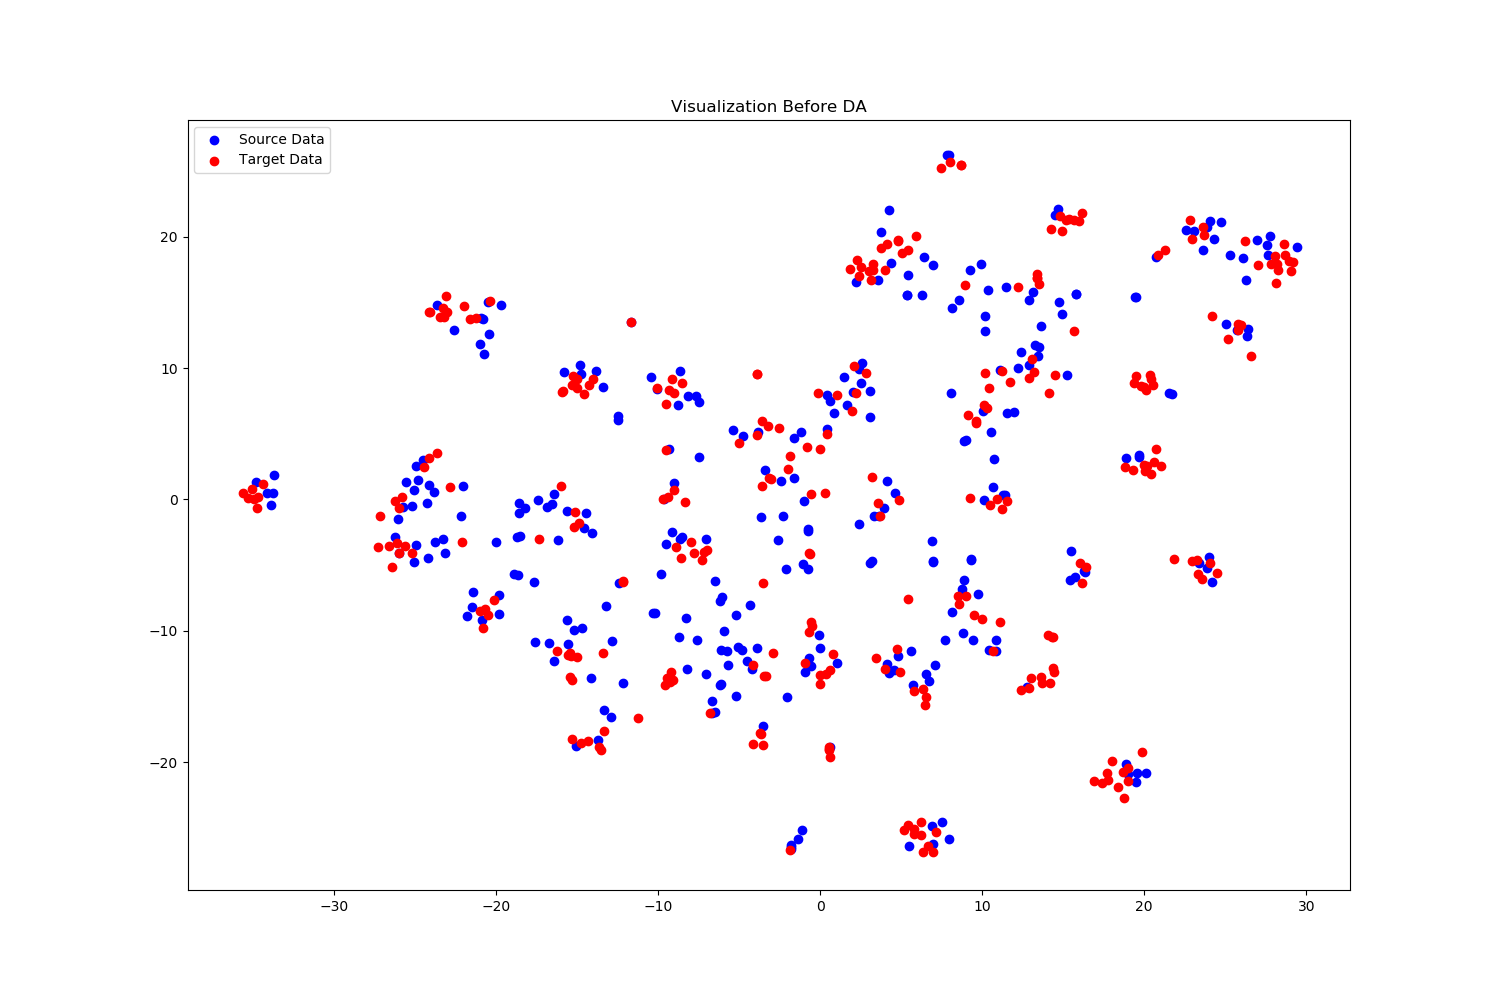
\includegraphics[width=1.5in, height=1.5in]{Ldann/std_P2R/before.png}
\end{minipage}%
\begin{minipage}[t]{0.2\textwidth}
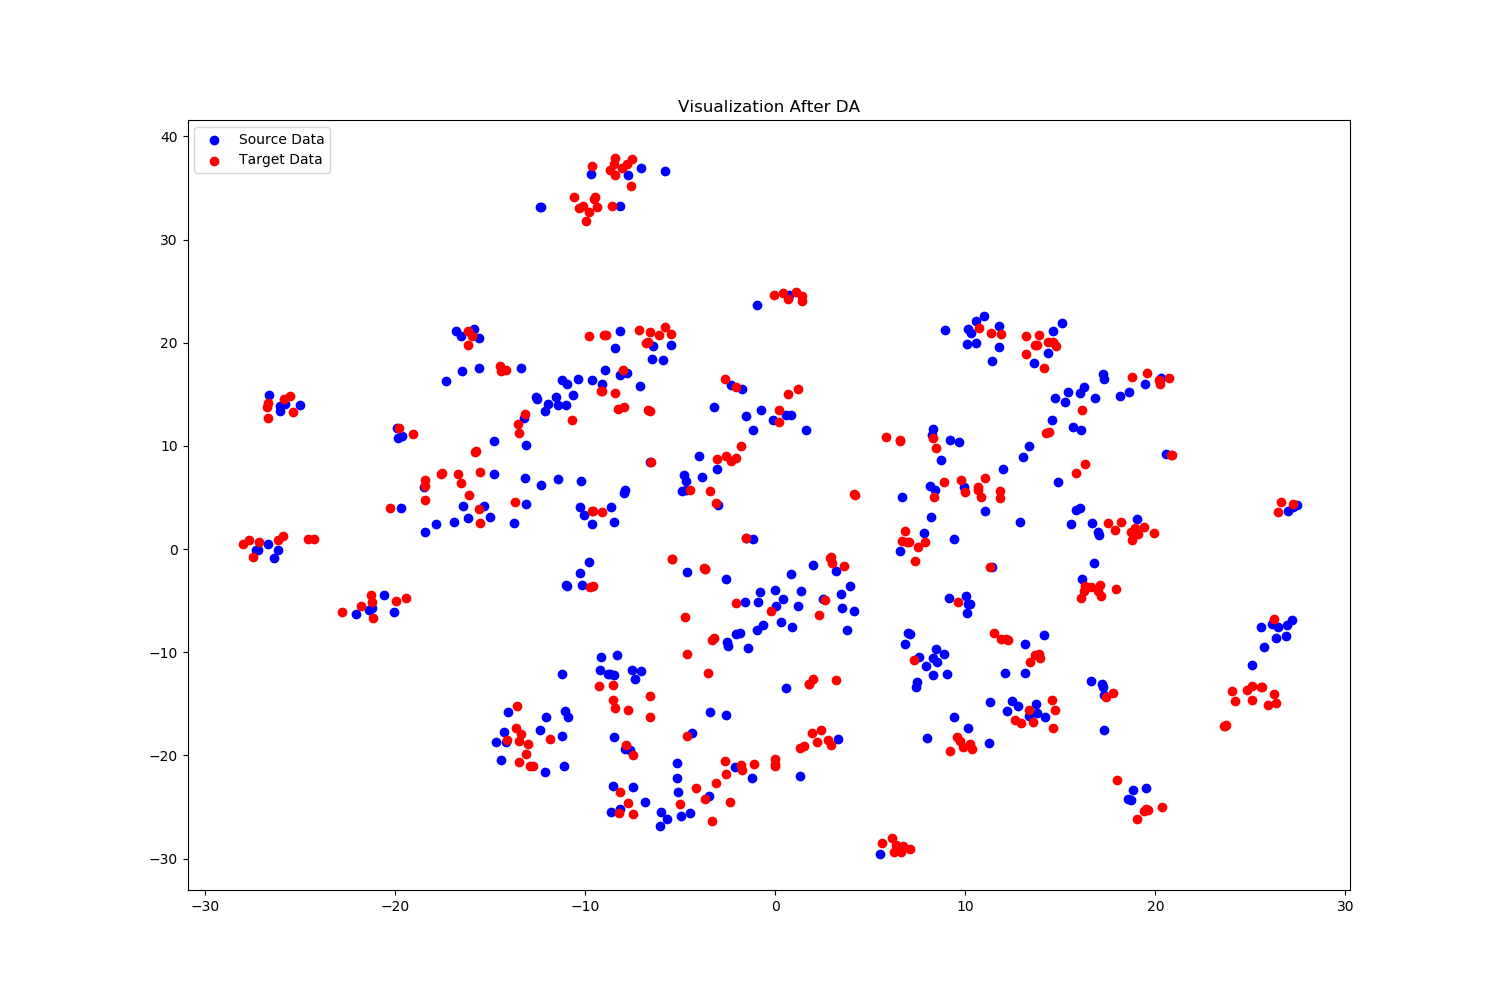
\includegraphics[width=1.5in, height=1.5in]{Ldann/std_P2R/after.png}
\end{minipage}%
\begin{minipage}[t]{0.45\textwidth}
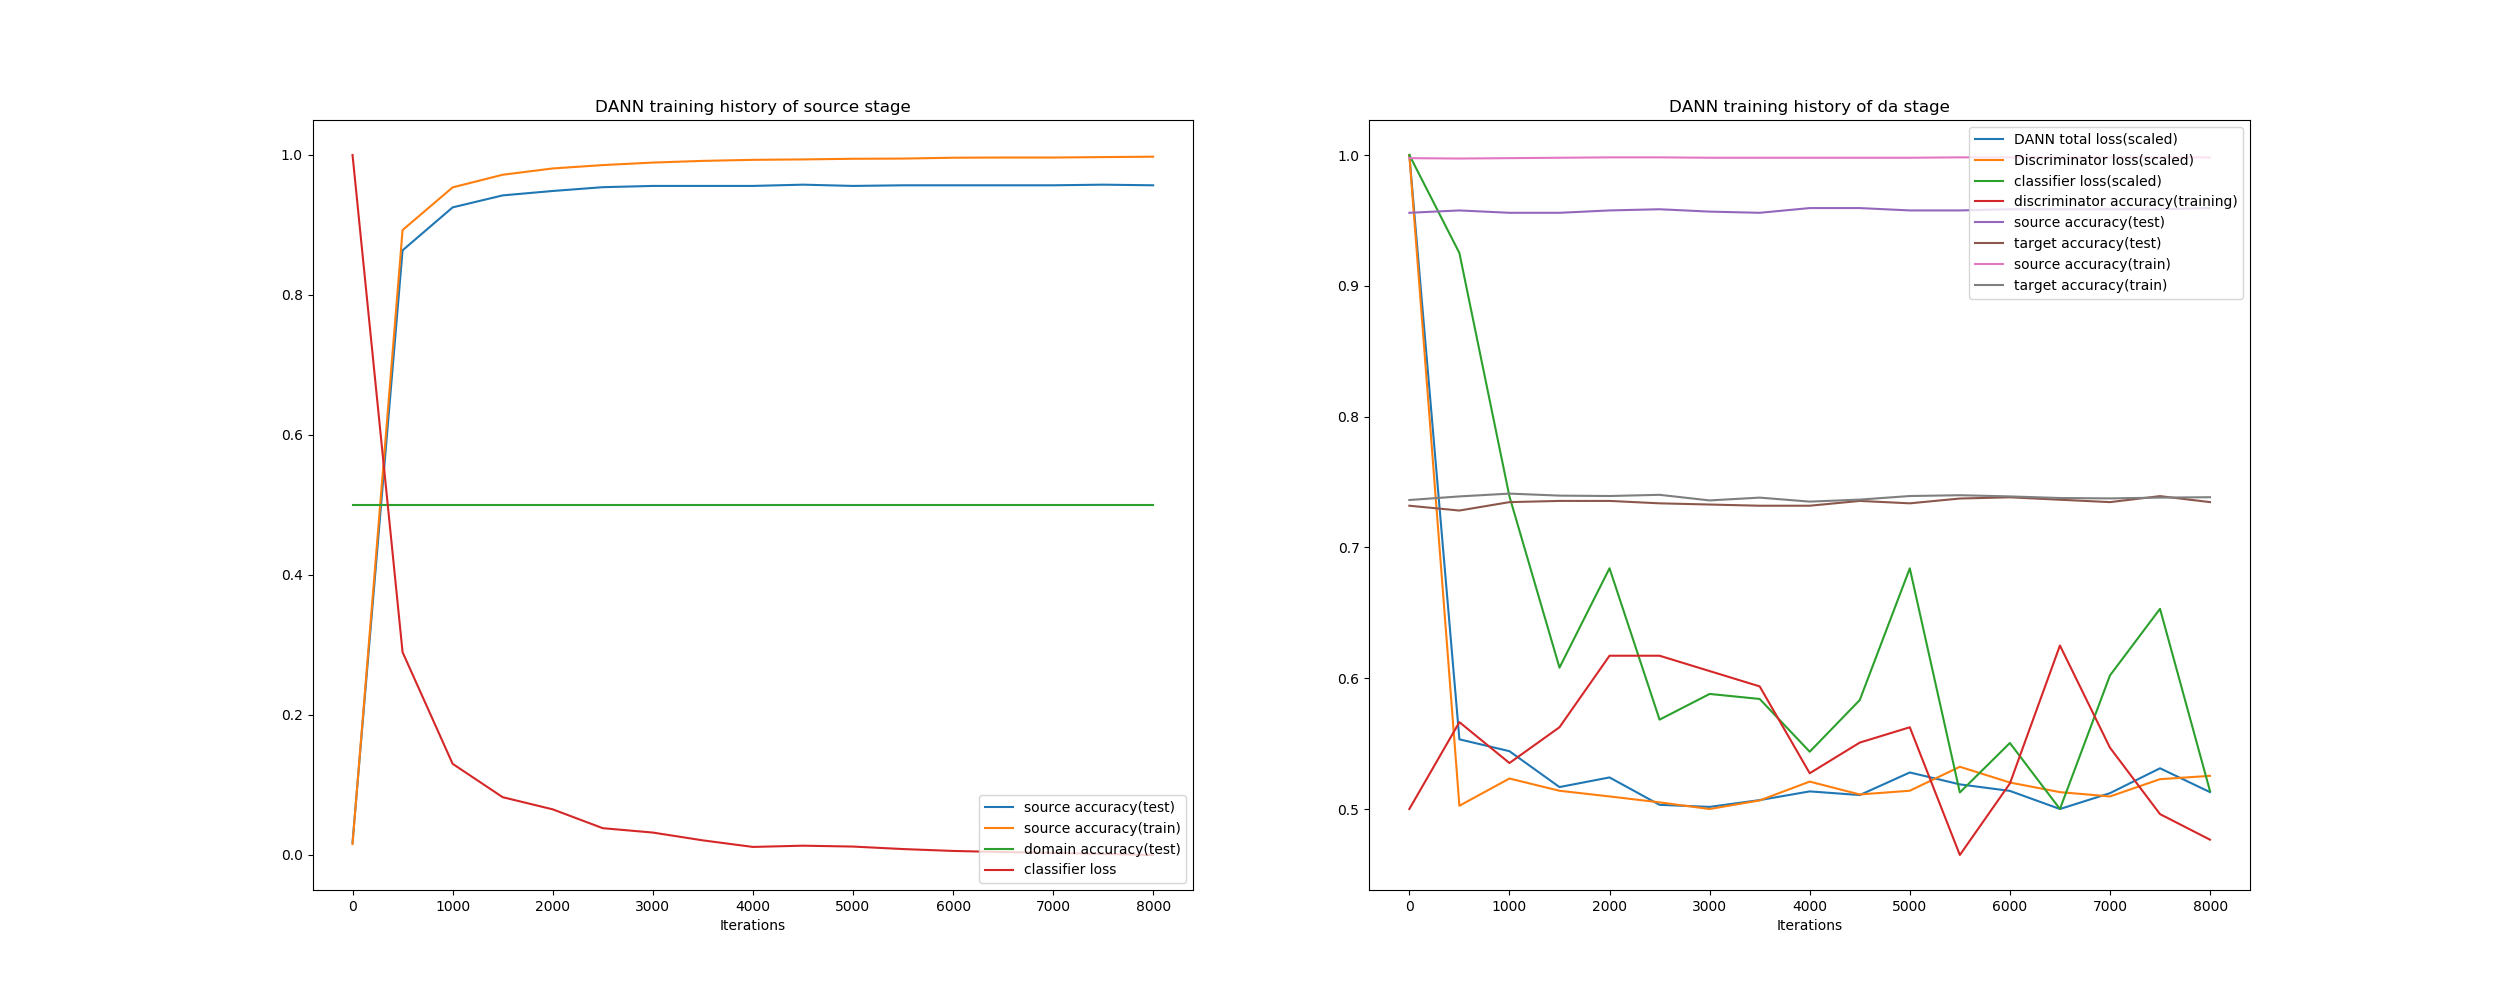
\includegraphics[width=3.5in, height=1.5in]{Ldann/std_P2R/dann.png}
\end{minipage}%
\caption{Visualization of DANN ExP Result}\label{fig:ExP2}
\end{figure*}

\section{Discussions}
\subsection{Problems of Network Design}
No matter which deep model we applied, severe overfitting occurs when training the classifier. Take ADDA for example, $Ac(M_s(X^{tr}_s))$ are always greater than $Ac(M_s(X^{te}_s))$ by about 0.15. We tried dropping out some neurons and increases L2 regularization constraint, but these measures do not ease overfitting but brings negative effects on $Ac(M_s(X^{te}_s))$.

Besides, specifically for ADDA, we found the discriminator can really grow too powerful to distinguish $X_s$ and $X_t$. We can design a more complicated and powerful $M$ to deceive the discriminator, of course. But a more complicated $M$ can also bring difficulties for the classification work.

And, it should be noticed that the visualization doesn't show an obvious effect after domain adaptation and the performance gain using domain adaptation is also poor, $0.004 \leq g \leq 0.013$. We think there can still be room for improvement.


\section{Conclusion}
Conclusions.


\section*{References}

Please number citations consecutively within brackets \cite{b1}. The
sentence punctuation follows the bracket \cite{b2}.

\begin{thebibliography}{00}
\bibitem{ADDA1} Eric Tzeng, Judy Hoffman, Kate Saenko and Trevor Darrel, ``Adversarial Discriminative Domain Adaptation''.
\bibitem{DANN1} Yaroslav Ganin, Evgeniya Ustinova, Hana Ajakan, Pascal Germain, Hugo Larochelle, Francois Laviolette,
    Mario Marchand, Victor Lempitsky, ``Domain-Adversarial Training of Neural Networks''.
\end{thebibliography}
\vspace{12pt}
\color{red}
IEEE conference templates contain guidance text for composing and formatting

\end{document}
